\documentclass[a4paper,12pt,twoside]{article}
\usepackage[left=1in,right=1in,top=1in,bottom=1in]{geometry}

\usepackage{xeCJK}
\setCJKmainfont{Songti TC}
\setCJKfamilyfont{kai}{Songti TC}
\newcommand{\kai}{\CJKfamily{kai}} % 用 \kai{使用楷書}

\usepackage{lmodern}
\usepackage{titling}
\usepackage{titlesec}
\usepackage{graphicx}
\usepackage{float}
\usepackage{amsmath, amsthm, amssymb, amsfonts, mathrsfs}
\usepackage{upgreek} % 直立的希臘字母

\usepackage[shortlabels]{enumitem}
\usepackage{setspace}
\renewcommand{\baselinestretch}{1.5}
\usepackage[colorlinks]{hyperref}
\usepackage{fancyvrb}
\usepackage{fancyhdr}
\usepackage{multicol}
\usepackage{caption}
\usepackage{subcaption}
\usepackage{listings}
\usepackage{bm}
\usepackage{bbm} % for \mathbbm{1} (indicator function)
\usepackage{centernot}
\usepackage{mdframed}
\usepackage{xltabular}
\usepackage{tcolorbox}
\tcbuselibrary{skins, breakable}
\usepackage{tikz}
\usetikzlibrary{patterns, arrows.meta, positioning, calc, decorations.pathmorphing, decorations.pathreplacing, decorations.markings, decorations.shapes, angles, quotes, 3d, matrix}
\usepackage[nameinlink, capitalise]{cleveref}
\usepackage{diagbox}
\usepackage{booktabs}
\usepackage{multirow,array}
\usepackage{tabularx}
\usepackage{mathtools}
\usepackage{indentfirst} % 首段 indent
\setlength{\parindent}{2em}
\usepackage{cancel} % 數學式子畫線槓掉
\newcommand\mcancel[2][red]{\setbox0=\hbox{$#2$}%
\rlap{\raisebox{.45\ht0}{\textcolor{#1}{\rule{\wd0}{1pt}}}}#2}
\setcounter{MaxMatrixCols}{20}
\usepackage{datetime2}
\usepackage{paracol}

\makeatletter
\def\tiangan#1{\expandafter\@tiangan\csname c@#1\endcsname}
\def\@tiangan#1{%
  \ifcase#1\or (甲)\or (乙)\or (丙)\or (丁)\or (戊)\or (己)\or (庚)\or (辛)\or (壬)\or (癸)\else(?)\fi
}
\AddEnumerateCounter{\tiangan}{\@tiangan}{(甲)}
\makeatother

% 支援 \wideparen 圓弧記號（若未載入 yhmath，可用此巨集穩定渲染）
\providecommand{\wideparen}[1]{\overset{\frown}{#1}}
\providecommand{\redtext}[1]{{\color{red} #1}}
\providecommand{\bluetext}[1]{{\color{blue} #1}}

\AtBeginDocument{%
 \setlength{\abovedisplayskip}{6pt}
 \setlength{\belowdisplayskip}{6pt}
 \setlength{\abovedisplayshortskip}{4pt}
 \setlength{\belowdisplayshortskip}{4pt}
}

\definecolor{codegreen}{rgb}{0,0.6,0}
\definecolor{codegray}{rgb}{0.5,0.5,0.5}
\definecolor{codepurple}{rgb}{0.58,0,0.82}
\definecolor{backcolour}{rgb}{0.95,0.95,0.92}

\lstdefinestyle{mystyle}{
 backgroundcolor=\color{backcolour},
 commentstyle=\color{codegreen},
 keywordstyle=\color{magenta},
 numberstyle=\tiny\color{codegray},
 stringstyle=\color{codepurple},
 basicstyle=\ttfamily\footnotesize,
 breakatwhitespace=false,
 breaklines=true,
 captionpos=b,
 keepspaces=true,
 numbers=left,
 numbersep=5pt,
 showspaces=false,
 showstringspaces=false,
 showtabs=false,
 tabsize=2
}
\lstset{style=mystyle}

\hypersetup{citecolor=blue, linkcolor=blue, urlcolor=blue}

\DeclareMathOperator{\supp}{supp}
\DeclareMathOperator{\skewness}{Skewness}
\DeclareMathOperator{\DU}{D-U}
\DeclareMathOperator{\CU}{C-U}
\DeclareMathOperator{\Geo}{Geo}
\DeclareMathOperator{\Pois}{Pois}
\DeclareMathOperator{\Gam}{Gam}
\DeclareMathOperator{\LN}{LogN}
\DeclareMathOperator{\cov}{Cov}
\DeclareMathOperator*{\argmax}{arg\,max}
\DeclareMathOperator*{\argmin}{arg\,min}
\DeclareMathOperator{\re}{Re}
\DeclareMathOperator{\im}{Im}

\newcommand{\N}{\mathbb{N}}
\newcommand{\Z}{\mathbb{Z}}
\newcommand{\Q}{\mathbb{Q}}
\newcommand{\R}{\mathbb{R}}
\newcommand{\C}{\mathbb{C}}
\newcommand{\G}{\mathcal{G}}
\newcommand{\mP}{\mathbb{P}}
\newcommand{\F}{\mathcal{F}}
\newcommand{\B}{\mathcal{B}}
\newcommand{\1}{\mathbbm{1}}
\newcommand{\Poi}{\text{Poi}}
\newcommand{\Var}{\text{Var}}
\newcommand{\as}{\text{a.s.}}
\newcommand{\vect}[1]{\boldsymbol{\mathbf{#1}}}
\newcommand{\paren}[1]{\left({#1}\right)}
\newcommand{\brk}[1]{\left[{#1}\right]}
\newcommand{\curl}[1]{\left\{{#1}\right\}}
\providecommand{\lambdaup}{\uplambda}
\renewcommand{\lambda}{\lambdaup}
\providecommand{\wideparen}[1]{\overset{\frown}{#1}}

\theoremstyle{definition} % 定理環境 style 改用正體
\newtheorem{theorem}{定理}
\newtheorem*{theorem*}{定理}
\newtheorem{definition}{定義}
\newtheorem*{definition*}{定義}
\newtheorem{example}{例子}
\newtheorem*{example*}{例子}
\newtheorem{exercise}{練習}
\newtheorem*{exercise*}{練習}
\newtheorem{corollary}{推論}
\newtheorem*{corollary*}{推論}
\newtheorem{property}{性質}
\newtheorem*{property*}{性質}
\newtheorem{prop}{命題}
\newtheorem*{prop*}{命題}
\newtheorem{proposition}[prop]{命題}
\newtheorem*{proposition*}{命題}
\newtheorem{lemma}{引理}
\newtheorem*{lemma*}{引理}
\newtheorem{problem}{問題}
\newtheorem*{problem*}{問題}
\newtheorem*{remark}{註}
\newtheorem{discussion}{論例}
\newtheorem*{discussion*}{論例}
\newtheorem{homework}{作業}
\newtheorem*{homework*}{作業}
\newtheorem{example-non}{例}

% 讓 \begin{solution} 與 \begin{solution*} 皆可用，並以 # 或 \square 結尾
\newtheorem*{solution}{【解】}
\AtEndEnvironment{solution}{\hfill$\#$}

% 每章（\section）自動重置定理、例題、論例、命題、公式等計數器，確保全冊與單章編譯編號完全一致
\makeatletter
\@addtoreset{theorem}{section}
\@addtoreset{definition}{section}
\@addtoreset{example}{section}
\@addtoreset{exercise}{section}
\@addtoreset{corollary}{section}
\@addtoreset{property}{section}
\@addtoreset{prop}{section}
\@addtoreset{lemma}{section}
\@addtoreset{problem}{section}
\@addtoreset{discussion}{section}
\@addtoreset{homework}{section}
\@addtoreset{example-non}{section}
\@addtoreset{equation}{section}
\makeatother

% 當原書該章各節（§ X-Y）獨立重新起算定理、例題、論例、公式編號時，於 \subsection 後呼叫 \resetsectcounters
\newcommand{\resetsectcounters}{%
  \setcounter{theorem}{0}%
  \setcounter{definition}{0}%
  \setcounter{example}{0}%
  \setcounter{exercise}{0}%
  \setcounter{corollary}{0}%
  \setcounter{property}{0}%
  \setcounter{prop}{0}%
  \setcounter{lemma}{0}%
  \setcounter{problem}{0}%
  \setcounter{discussion}{0}%
  \setcounter{homework}{0}%
  \setcounter{example-non}{0}%
  \setcounter{equation}{0}%
}

\renewcommand{\figurename}{圖}
\renewcommand{\tablename}{表}

% 統一勘誤表返回連結巨集：各單章主檔與全冊主檔皆於勘誤表標題處定義 \label{sec:current_errata}
\providecommand{\errataref}{\hyperref[sec:current_errata]{目錄前勘誤表}}

\DeclareMathOperator{\var}{Var}
\DeclareMathOperator{\corr}{corr}
\DeclareMathOperator{\rank}{rank}
\DeclareMathOperator{\MSE}{MSE}
\DeclareMathOperator{\SSE}{SSE}
\DeclareMathOperator{\SST}{SST}
\DeclareMathOperator{\SSR}{SSR}
\DeclareMathOperator{\sgn}{sign}
\DeclareMathOperator{\alt}{Alt}
\DeclareMathOperator{\adj}{adj}
\DeclareMathOperator{\curlOp}{curl}
\DeclareMathOperator{\spn}{span}
\DeclareMathOperator{\sse}{SSE}
\DeclareMathOperator{\tr}{tr}

\newcommand{\ep}{\varepsilon}
\newcommand{\p}{\partial}
\newcommand{\abs}[1]{\left|#1\right|}
\newcommand\norm[1]{\left\lVert#1\right\rVert}
\newcommand{\innerprod}[1]{\langle#1\rangle}
\newcommand{\ds}{\displaystyle}
\newcommand{\blank}{\rule[-1mm]{1.5cm}{0.1mm}}
\newcommand{\dint}{\displaystyle\int}
\renewcommand{\bar}{\overline}

\newtheoremstyle{remark}{}{}{}{}{\bfseries\sffamily}{.}{.5em}{#1}
\theoremstyle{remark}

\newtheorem*{remark*}{\textit{Remark}}
\newtheorem*{solution*}{解}

\AtEndEnvironment{solution*}{\hfill$\square$}
\newtheorem*{hint*}{Hint}


\providecommand{\redtext}[1]{{\color{red} #1}}
\providecommand{\bluetext}[1]{{\color{blue} #1}}

\fancypagestyle{firstpage}{
  \fancyhf{}
  \fancyhead[R]{\small《高中數學實驗教材》第 6 冊（自然組）}
  \fancyhead[L]{\small 第 2 章\quad 方程式論}
  \fancyfoot[C]{\thepage}
}

\pagestyle{fancy}
\setlength{\headheight}{14pt}
\renewcommand{\headrulewidth}{0.5pt}
\renewcommand{\footrulewidth}{0pt}
\fancyhead{}
\fancyhead[LE]{\small 《高中數學實驗教材》第六冊（自然組）}
\fancyhead[RO]{\small 第二章\quad 方程式論}
\fancyfoot[C]{\thepage}

\title{\LARGE\textbf{《高中數學實驗教材》第六冊（自然組）}\\[0.5em] \Large\textbf{第二章\quad 方程式論}}
\author{\textbf{高中數學實驗教材編輯小組}\quad 編著}
\date{民國六十五年（1976）再版}

\begin{document}

\maketitle
\thispagestyle{firstpage}

% ==========================================
% 掃描檔勘誤、文字校訂與疑難處說明（依規則整理於目錄之前）
% ==========================================
\section*{【說明】第二章掃描檔勘誤、疑難處與文義校訂表}
\addcontentsline{toc}{section}{【說明】第二章掃描檔勘誤、疑難處與文義校訂表}
\label{sec:errata_notes_b6_ch2}
\label{sec:current_errata}

本章依據 1976 年再版《高中數學實驗教材 第六冊（自然組）》（高三下）第二章「方程式論」掃描原件完整轉錄為 \LaTeX{} 格式。為忠實反映教材原始內容並兼顧排版品質與嚴謹性，依作業規範將掃描檔中出現之印刷訛誤、符號缺漏、字模損毀、歷史印記雜訊及文義疑難處詳細考證彙整於下表。讀者可點擊表格中之章節連結直接跳至正文對應位置：

\begin{table}[H]
\centering
\small
\renewcommand{\arraystretch}{1.35}
\begin{tabularx}{\textwidth}{|p{3.2cm}|p{3.8cm}|X|}
\hline
\textbf{章節位置} & \textbf{掃描檔原始現象 / 誤植} & \textbf{考證說明與校訂處理} \\ \hline

\hyperref[note:b6-ch2-p95-trace]{§ II-3 頁 95 作業 7(i)} & 
「諸根之和為 $-(a_{11}+a_{22}+a_{33})$」 & 
原書特徵方程式展開後最高兩項為 $(-x)^3 + (a_{11}+a_{22}+a_{33})x^2$，依根與係數關係根之和應為首項係數除次高項係數取負，即 $a_{11}+a_{22}+a_{33}$，原書漏消負號，據此校訂。 \\ \hline

\hyperref[note:b6-ch2-p117-cubic-ineq]{§ II-5 頁 117 習題 II-5 第 6 題} & 
「$-4p^3r > 27r$」 & 
依三次方程式判別式 $\Delta = -4p^3 - 27r^2 > 0 \iff -4p^3 > 27r^2$，原書右式漏平方且左式印有雜訊 $r$，據實根條件加註說明。 \\ \hline

\end{tabularx}
\end{table}

\newpage
\renewcommand{\contentsname}{目\qquad 次}
\tableofcontents
\newpage

\setcounter{section}{1}
% !TeX root = Chapter2_main.tex
% =========================================================================
% 《高中數學實驗教材》第六冊（自然組）
% 第二章 方程式論
% =========================================================================
\section{方程式論}\label{sec:b6-ch2}

\begin{center}
\begin{minipage}{0.75\textwidth}
\begin{itemize}[leftmargin=2em, itemsep=0.3em]
  \item[§ II-1] \textbf{方程式論}
  \begin{itemize}[leftmargin=2em, itemsep=0.2em]
    \item[甲、] 一元 $n$ 次方程式
    \item[乙、] 插入法
  \end{itemize}
  \item[§ II-2] \textbf{代數的基本定理}
  \begin{itemize}[leftmargin=2em, itemsep=0.2em]
    \item[甲、] 複係數方程式
    \item[乙、] 實係數方程式
    \item[丙、] 函數之圖示
  \end{itemize}
  \item[§ II-3] \textbf{根與係數的關係與對稱式}
  \begin{itemize}[leftmargin=2em, itemsep=0.2em]
    \item[甲、] 根與係數的關係
    \item[*乙、] 對稱式基本定理
  \end{itemize}
  \item[§ II-4] \textbf{多項式函數的導數}
  \begin{itemize}[leftmargin=2em, itemsep=0.2em]
    \item[甲、] 導函數
    \item[乙、] 重根定理
    \item[丙、] 泰勒展開式
    \item[丁、] 函數的極大與極小
  \end{itemize}
  \item[*§ II-5] \textbf{三次方程式、四次方程式的解法}
  \begin{itemize}[leftmargin=2em, itemsep=0.2em]
    \item[甲、] 一元三次方程式的解法
    \item[乙、] 一元四次方程式的解法
  \end{itemize}
  \item[附錄 III] \textbf{結式判別式與史篤姆定理}
\end{itemize}
\end{minipage}
\end{center}

\begin{center}
$* \qquad * \qquad * \qquad * \qquad *$
\end{center}

\subsection{方程式論}\label{sec:b6-2-1}

我們在前五冊裡已經介紹了許多函數，如多項式函數、三角函數、指數函數等。給定一函數 $y=f(x)$，可以明確地在 $xy$ 平面上做一相對應的圖形如圖：

\begin{figure}[H]
\centering
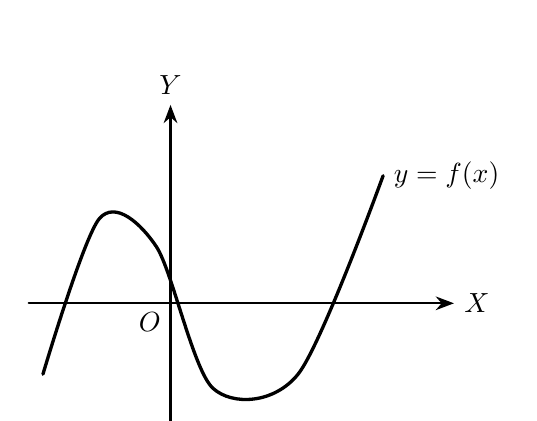
\begin{tikzpicture}[>=Stealth, scale=0.9, line cap=round, line join=round]
  \draw[->, thick] (-2.0, 0) -- (4.0, 0) node[right] {$X$};
  \draw[->, thick] (0, -1.8) -- (0, 2.8) node[above] {$Y$};
  \node[below left] at (0,0) {$O$};

  % Cubic curve crossing x axis 3 times
  \draw[very thick, smooth] plot coordinates {(-1.8, -1.0) (-1.0, 1.2) (-0.2, 0.8) (0.6, -1.2) (1.8, -1.0) (3.0, 1.8)} node[right] {$y=f(x)$};
\end{tikzpicture}
\end{figure}

此圖形與 $x$ 軸的交點在那裡？有多少交點？這些問題以代數的講法就是解聯立方程式
\[ \begin{cases} y = f(x) \\ y = 0 \end{cases} \]
此聯立方程式可以更簡便地記作 $f(x)=0$，而稱為\textbf{方程式}。如
\begin{align*}
\text{指數方程式：}& 5^{x+1} - 3 = 0, \\
\text{三角方程式：}& \sin 2x - 1 = 0, \\
\text{整式方程式：}& 5x^2 + 7x + 1 = 0, \\
\text{分式方程式：}& \dfrac{5x^2+7}{x+1} + \dfrac{6x+1}{x^3+1} + 1 = 0 \text{。}
\end{align*}
求滿足方程式中未知數的值就是解方程式。在方程式論裡我們只討論\textbf{多項式方程式}的求解。

要注意：函數討論的重點在於變量 $x$ 與 $y$ 間的關係，而相應的方程式 $f(x)=0$ 另有不同的意義。當然函數 $y=f(x)$ 與方程式 $f(x)=0$ 之間有相當密切的關係，二者在本章節中經常相互出現。又我們常把多項式與多項式函數二名稱不給以區別。讀者必能容易看出前者 $y=a_0 x^n + a_1 x^{n-1} + \dots + a_n$ 只表示 $x$ 為不定元，而用加，乘做出來的式子，後者意味著有函數對應關係，即給定一 $x=a$ 之值，有一確定的 $y$ 值與之對應。在實係數或複係數上此二者可以不加以區別的。

\subsubsection*{甲、一元 n 次方程式}\label{subsec:b6-2-1-a}

任給一多項式 $f(x) = a_n x^n + a_{n-1} x^{n-1} + \dots + a_1 x + a_0$，其中 $a_n \ne 0$，則 $f(x)=0$ 稱為\textbf{一元 $n$ 次方程式}。根據這樣的定義，我們可以寫出 $n=1, 2, 3, 4, \dots$ 時的一元方程式：
\begin{align*}
\text{一次的：}& a_1 x + a_0 = 0 \\
\text{二次的：}& a_2 x^2 + a_1 x + a_0 = 0 \\
\text{三次的：}& a_3 x^3 + a_2 x^2 + a_1 x + a_0 = 0 \\
&\dots\dots\dots\dots
\end{align*}
一元 $n$ 次方程式論的中心課題在於討論根的求法，根與係數的關係等。因此對於其係數所在的範圍必須要有較明確的說明。為區別起見，當係數 $a_i$ ($i=0, \dots, n$) 皆為複數，稱為\textbf{複係數方程式}，當係數 $a_i$ 皆為實數，則稱為\textbf{實係數方程式}，仿此，如果 $a_i$ 皆為有理數，則稱為\textbf{有理係數方程式}。顯然

\begin{center}
\begin{tikzpicture}[>=Stealth, scale=0.9, line cap=round, line join=round]
  % Ellipse: 複係數方程式
  \draw[thick] (1.6, 0.9) ellipse (1.6cm and 0.78cm);
  \node at (1.6, 0.9) {複係數方程式};

  \node at (3.75, 0.9) {$\supset$};

  % Rectangle: 實係數方程式
  \draw[thick] (4.3, 0.12) rectangle (7.4, 1.68);
  \node at (5.85, 0.9) {實係數方程式};

  \node at (7.95, 0.9) {$\supset$};

  % Triangle: 有理係數方程式 (matching original p.82)
  \draw[thick] (8.45, 0.02) -- (12.25, 0.02) -- (10.35, 2.02) -- cycle;
  \node[align=center, font=\small] at (10.35, 0.68) {有理\\係數方程式};
\end{tikzpicture}
\end{center}

本章中如無特別指明係數所在的範圍，則所討論者皆為複係數方程式。

\begin{definition}\label{def:b6-2-1}
對於 $n$ 次方程式 $f(x) = a_n x^n + a_{n-1} x^{n-1} + \dots + a_0 = 0$ 若有一數 $\alpha$，使得
\[ f(\alpha) = a_n \alpha^n + a_{n-1} \alpha^{n-1} + \dots + a_0 = 0 \]
則稱 $\alpha$ 為此方程式之\textbf{一根}。
\end{definition}

第一冊第五章所講的餘式定理，可推廣至複係數多項式。其中一個重要的推論可重述如下：

\begin{corollary}[因式定理]\label{cor:b6-2-1}
設 $f(x)=0$ 為 $n$ 次方程式，若 $\alpha$ 為 $f(x)=0$ 之一根，則 $f(x)$ 能被 $x-\alpha$ 整除，反之若 $f(x) = (x-\alpha)g(x)$，（$g(x)$ 為一多項式）則 $\alpha$ 為 $f(x)=0$ 之一根。
\end{corollary}

\begin{example}\label{ex:b6-2-1}
已知 1 與 7 均為方程式 $x^4 - 17x^3 + 99x^2 - 223x + 140 = 0$ 之一根，試解此方程式。
\end{example}

\paragraph{【解】}
利用綜合除法，以 $x-1$ 除方程式之左端，再以 $x-7$ 除，其商如下：
\begin{center}
\renewcommand{\arraystretch}{1.2}
\begin{tabular}{rrrrr|r}
$1$ & $-17$ & $99$ & $-223$ & $140$ & $1$ \\
    & $+1$  & $-16$ & $+83$ & $-140$ & \\
\hline
$1$ & $-16$ & $83$ & $-140$ & $0$ & $7$ \\
    & $+7$  & $-63$ & $+140$ & & \\
\hline
$1$ & $-9$  & $20$ & $0$ & &
\end{tabular}
\end{center}
由此得
\begin{align*}
x^4 - 17x^3 + 99x^2 - 223x + 140 &= (x-1)(x-7)(x^2 - 9x + 20) \\
&= (x-1)(x-7)(x-4)(x-5)
\end{align*}
故其根有 $1, 7, 4, 5$。\hfill$\#$

\begin{example}\label{ex:b6-2-2}
求一三次多項式函數 $y=f(x)$，使得 $f(1)=0, f(4)=0, f(-1)=0, f(3)=8$。
\end{example}

\paragraph{【解】}
設此函數為
\begin{equation}
f(x) = a_3 x^3 + a_2 x^2 + a_1 x + a_0 \label{eq:b6-2-1-1}
\end{equation}
根據推論 1 知
\begin{equation}
f(x) = c(x-1)(x-4)(x+1) \label{eq:b6-2-1-2}
\end{equation}
\[ 8 = f(3) = c(3-1)(3-4)(3+1) \]
得 $c = -1$。故所求的函數為
\begin{align*}
f(x) &= (-1)(x-1)(x-4)(x+1) \\
&= -x^3 + 4x^2 + x - 4
\end{align*}
\hfill$\#$

\subsubsection*{作業 1}\label{hw:b6-2-1}
試解 $x - 9\sqrt{x} - 20 = 0$。

\subsubsection*{作業 2}\label{hw:b6-2-2}
試求三次多項式 $y=f(x)$ 滿足 $f(1)=0, f(3)=0, f(-1)=0, f(4)=2$。

\subsubsection*{乙、插入法}\label{subsec:b6-2-1-b}

三、四冊已說明兩點決定唯一一直線，即決定一個一次函數 $y=mx+b$，上段例 2 又述及給定四點 $(1, 0), (4, 0), (-1, 0), (3, 8)$，則可得一三次多項式其圖形通過此四點。我們不免聯想到：如果在平面上給定不同的 $n$ 個點 $(a_1, b_1), \dots, (a_n, b_n)$ 可否尋得一個 $n-1$ 次多項式 $f(x)$，使得 $f(a_i)=b_i$ 呢？現在先以三點為例：

假設 $(a_1, b_1), (a_2, b_2), (a_3, b_3)$ 為給定三點，$a_1, a_2, a_3$ 互異。首先假設
\[ g_1(x) = c_1(x-a_2)(x-a_3) \]
其中 $c_1$ 為未定常數，我們希望適當地取 $c_1$ 使得 $g_1(a_1)=b_1$，如此必然要有
\[ c_1 = \dfrac{b_1}{(a_1-a_2)(a_1-a_3)} \]
同理另外可取定二函數 $g_2(x), g_3(x)$ 為
\begin{align*}
g_2(x) &= \dfrac{b_2(x-a_1)(x-a_3)}{(a_2-a_1)(a_2-a_3)}, \quad g_2(a_2)=b_2, \quad g_2(a_1)=g_2(a_3)=0 \\
g_3(x) &= \dfrac{b_3(x-a_2)(x-a_1)}{(a_3-a_2)(a_3-a_1)}, \quad g_3(a_3)=b_3, \quad g_3(a_1)=g_3(a_2)=0
\end{align*}
令 $f(x) = g_1(x) + g_2(x) + g_3(x)$，則 $f(x)$ 為所求的二次式，因為
\begin{align*}
f(a_1) &= g_1(a_1) + g_2(a_1) + g_3(a_1) = g_1(a_1) + 0 + 0 = b_1 \\
f(a_2) &= g_1(a_2) + g_2(a_2) + g_3(a_2) = 0 + g_2(a_2) + 0 = b_2 \\
f(a_3) &= g_1(a_3) + g_2(a_3) + g_3(a_3) = 0 + 0 + g_3(a_3) = b_3
\end{align*}
上述的方法稱為 \textbf{Lagrange（拉格蘭日）插入法}，推廣到 $n$ 點的情形則為：

\begin{theorem}[Lagrange's 插入法]\label{thm:b6-2-lagrange}
設 $a_1, \dots, a_n$ 為 $n$ 個不同數，$b_1, \dots, b_n$ 為另一組 $n$ 個數。令
\[ P_i(x) = b_i \dfrac{(x-a_1)\dots(x-a_{i-1})(x-a_{i+1})\dots(x-a_n)}{(a_i-a_1)\dots(a_i-a_{i-1})(a_i-a_{i+1})\dots(a_i-a_n)} \]
則
\[ f(x) = P_1(x) + \dots + P_i(x) + \dots + P_n(x) \]
為 $n-1$ 次多項式且滿足 $f(a_i)=b_i, \quad i=1, \dots, n$。
\end{theorem}

\begin{example}\label{ex:b6-2-3}
求一次數最低的多項式 $f(x)$ 使能滿足 $f(-1)=-6, f(0)=2, f(1)=-2, f(2)=6$。
\end{example}

\paragraph{【解】}
令
\begin{align*}
P_1(x) &= \dfrac{-6(x-0)(x-1)(x-2)}{(-1-0)(-1-1)(-1-2)} = x(x-1)(x-2) \\
P_2(x) &= \dfrac{2(x+1)(x-1)(x-2)}{(0+1)(0-1)(0-2)} = (x+1)(x-1)(x-2) \\
P_3(x) &= \dfrac{-2(x+1)(x-0)(x-2)}{(1+1)(1-0)(1-2)} = (x+1)x(x-2) \\
P_4(x) &= \dfrac{6(x+1)(x-0)(x-1)}{(2+1)(2-0)(2-1)} = (x+1)x(x-1)
\end{align*}
則
\begin{align*}
f(x) &= x(x-1)(x-2) + (x+1)(x-1)(x-2) \\
&\quad + (x+1)x(x-2) + (x+1)x(x-1) \text{ 為所求。}
\end{align*}
\hfill$\#$

\subsubsection*{作業 3}\label{hw:b6-2-3}
試求一多項式 $f(x)$ 使能滿足 $f(1)=6, f(2)=3, f(-1)=-2, f(0)=1$。

\subsubsection*{習題 II-1}\label{sec:b6-ex2-1}

\begin{enumerate}[label=\arabic*., leftmargin=2em]
  \item 令 $f(x)=a_0 x^n + \dots + a_n$，試證下列各題：
  \begin{enumerate}[label=(\roman*)]
    \item 若 $a_n=0$，則 $f(x)=0$ 有一根為 0，若 $a_n=a_{n-1}=0$ 則 $f(x)=0$ 有二根為 0，餘類推。
    \item 若 $a_0+a_1+\dots+a_n=0$，則 $f(x)=0$ 有 1 的根。
    \item 若 $a_0-a_1+\dots+(-1)^n a_n=0$，則 $f(x)=0$ 有 $-1$ 的根。
    \item 若 $a_i \ge 0$ ($i=0, 1, \dots, n$)，則 $f(x)=0$ 無正根。
    \item 若 $f(x)$ 的各項係數為正負相間，則 $f(x)=0$ 無負根。
  \end{enumerate}

  \item 試證 5 為 $f(x)=x^3-28x+15=0$ 的一根，試解 $f(x)=0$。

  \item 已知 $f(x)=0$ 有 $2, 1+i, 1-i$ 三根，$f(1)=2$ 試求 $f(x)$。

  \item 試證 $2x^3+3x^2-4x+5=0$ 的各根不大於 1。

  \item 試證 $x^3-2x^2-2x+1=0$ 及 $x^4-7x^2+1=0$ 有二根相同，並求各根。

  \item 解 $x^4+8x^3+18x^2-27=0$。

  \item 解 $(x-a)(x+2a)(x-3a)(x+4a)-24a^4=0$。

  \item 解 $x(x-1)(x-2)(x-3)-4 \cdot 3 \cdot 2 \cdot 1=0$。

  \item 解 $(a-x)^4+(x-b)^4-(a-b)^4=0$。

  \item 解
  \[ x^3 - a^3 \dfrac{(x-b)(x-c)}{(a-b)(a-c)} - b^3 \dfrac{(x-c)(x-a)}{(b-c)(b-a)} - c^3 \dfrac{(x-a)(x-b)}{(c-a)(c-b)} = 0 \]

  \item 試求滿足下列各條件次數最低的多項式：
  \begin{enumerate}[label=(\roman*)]
    \item $f(-1)=3, f(2)=f(1)=f(-5)=0$。
    \item $f(1)=2, f(2)=3, f(3)=4, f(4)=5$。
  \end{enumerate}

  \item 設 $c_1, \dots, c_k$ 為不同之數，取一 $j \in \{1, 2, \dots, k\}$ 令
  \[ p_j(x) = \dfrac{(x-c_1)\dots(x-c_{j-1})(x-c_{j+1})\dots(x-c_k)}{(c_j-c_1)\dots(c_j-c_{j-1})(c_j-c_{j+1})\dots(c_j-c_k)} \]
  \begin{enumerate}[label=(\roman*)]
    \item 試證 $x = c_1 p_1(x) + c_2 p_2(x) + \dots + c_k p_k(x)$。
    \item 設 $g(x)$ 為次數小於 $k-1$ 之多項式，則
    \[ g(x) = g(c_1)p_1(x) + \dots + g(c_k)p_k(x) \]
  \end{enumerate}
\end{enumerate}

\subsection{代數的基本定理}\label{sec:b6-2-2}
\resetsectcounters

\subsubsection*{甲、複係數方程式}\label{subsec:b6-2-2-a}

令 $f(x) = a_n x^n + a_{n-1} x^{n-1} + \dots + a_0 = 0$ 為 $n$ 次方程式，由因式定理知如果 $c_1, c_2, \dots, c_r$ 為 $f(x)$ 之根，則
\[ f(x) = (x-c_1)(x-c_2)\dots(x-c_r)f_r(x) \]
比較兩邊的次數，得 $f_r(x)$ 為 $n-r$ 次多項式。這樣的 $f_r(x)=0$ 稱為 $f(x)=0$ 的\textbf{降冪方程式}。如果 $c_{r+1}$ 是 $f_r(x)=0$ 之一根，再用一次因式定理於 $f_r(x)=0$，得
\[ f(x) = (x-c_1)\dots(x-c_r)(x-c_{r+1})f_{r+1}(x) \]
所以降冪方程式的根，仍是原方程式的根。

\begin{theorem}\label{thm:b6-2-roots-bound}
設 $f(x)$ 為一個 $n$ 次多項式，則 $f(x)=0$ 至多有 $n$ 個根。
\end{theorem}

\begin{proof}[【證明】]
因為一個 $n$ 次多項式，不能被一個 $n+1$ 次的多項式整除。
\end{proof}\hfill$\#$

上面的結論仍然有缺點，因不能得知方程式的根是否存在。大家都知道 $x^2+1=0$ 沒有實數根（因為實數的平方永遠為非負，加 1 後絕不等於 0），如果擴大數的範圍，則可設一「數」$i$ 滿足此方程式。但是這僅是一個特例，方程式有無很多，是否每次都得把數的範圍無窮次地擴展，引進新的數做為它們的根呢？這問題在十八世紀已由大數學家\textbf{高斯（Gauss）}得到解決，今述之如下。定理的證明（現已有很多種），需要更多的數學工具，而超出本書之範圍，故予從略。

\begin{theorem}[代數的基本定理]\label{thm:b6-2-fta}
令 $f(x)$ 為 $n$ 次多項式，則 $f(x)=0$ 至少有一複數為其根。
\end{theorem}

\begin{corollary}\label{cor:b6-2-n-roots}
$n$ 次方程式 $f(x)=0$ 恰有 $n$ 個複數根。
\end{corollary}

\begin{discussion}\label{disc:b6-2-1}
任一複數開平方仍然是複數。
\end{discussion}

\begin{proof}[【證明】]
複數 $a+bi$ ($ab \ne 0$) 開平方，就是要求 $x^2-(a+bi)=0$ 的根。根據推論 1 知此方程式有兩個複數根。實際上 $\sqrt{a+bi}$ 的求法是這樣的，設
\[ \sqrt{a+bi} = x+yi \]
兩邊平方，得
\[ a+bi = (x+yi)^2 = x^2-y^2 + 2xyi \]
故有
\[ \begin{cases} a = x^2-y^2 \\ b = 2xy \end{cases} \]
求解此聯立方程式，得二組 $x, y$（第四冊第五章複數系已述及）。
\end{proof}\hfill$\#$

\begin{example}\label{ex:b6-2-4}
試求 $z^2+5z+a+bi=0$ 有二實根之充要條件，其中 $a, b$ 為實數。
\end{example}

\paragraph{【解】}
其根為
\[ z = \dfrac{-5 \pm \sqrt{25 - 4(a+bi)}}{2} \]
此為實數當且僅當 $\sqrt{25 - 4(a+bi)}$ 為實數。設 $\sqrt{25 - 4(a+bi)} = x$，若 $x$ 為實數，則因
\[ 25 - 4a - 4bi = x^2 \]
必有 $b=0$ 及 $25-4a = x^2 \ge 0 \implies \dfrac{25}{4} \ge a$。故其充要條件為 $b=0, \dfrac{25}{4} \ge a$。\hfill$\#$

\subsubsection*{作業 4}\label{hw:b6-2-4}
\begin{enumerate}[label=(\roman*), leftmargin=2em]
  \item 求 $\sqrt{1+i}$。
  \item 已知方程式 $x^3 - (i+1)x^2 + (i-20)x + 20i = 0$ 有一根為 5，求解此方程式。
  \item 已知方程式 $x^2 + 2(1+i)x + a + bi = 0$ 有一實根為 2，試求 $a, b$ 且解此方程式。
\end{enumerate}

\subsubsection*{乙、實係數方程式}\label{subsec:b6-2-2-b}

$a+bi$ ($a, b$ 為實數) 的共軛數為 $a-bi$，二數的乘積為 $a^2+b^2$，和為 $2a$，以此二數為根做一方程式得 $x^2 - 2ax + a^2 + b^2 = 0$，反之，設 $x^2 + Cx + D = 0$ 為一個二次實係數方程式，如果它有一複數根 $a+bi$，則其共軛數 $a-bi$ 亦必為它的一根，這一現象是下述定理的特例：

\begin{theorem}[虛根共軛定理]\label{thm:b6-2-conjugate}
實係數方程式 $a_n x^n + a_{n-1} x^{n-1} + \dots + a_1 x + a_0 = 0$ 若有一複數根 $a+bi$，則其共軛數 $a-bi$ 亦為其根，其中 $a, b$ 為實數。
\end{theorem}

\begin{proof}[【證明】]
我們知道：
\begin{enumerate}[label=(\roman*), leftmargin=2em]
  \item 二複數乘積的共軛數，等於各個共軛數的乘積：$\bar{z_1 z_2} = \bar{z}_1 \bar{z}_2$。推論可得 $\bar{z_1 z_2 \dots z_n} = \bar{z}_1 \bar{z}_2 \dots \bar{z}_n$。又 $\bar{az} = a\bar{z}, \quad a \in \mathbb{R}$。
  \item 二複數和之共軛數等於各個共軛數之和：$\bar{z_1 + z_2} = \bar{z}_1 + \bar{z}_2$。
\end{enumerate}
由 (i) (ii) 知
\begin{align*}
\bar{f(z)} &= \bar{a_n z^n + a_{n-1} z^{n-1} + \dots + a_0} \\
&= a_n (\bar{z})^n + a_{n-1} (\bar{z})^{n-1} + \dots + a_0 = f(\bar{z})
\end{align*}
如果 $\alpha = a+bi$ 為 $f(x)=0$ 之一根，則
\[ f(\alpha) = a_n \alpha^n + a_{n-1} \alpha^{n-1} + \dots + a_0 = 0 \]
因此
\begin{align*}
0 = \bar{0} = \bar{f(\alpha)} &= a_n (\bar{\alpha})^n + a_{n-1} (\bar{\alpha})^{n-1} + \dots + a_1 (\bar{\alpha}) + a_0 = f(\bar{\alpha})
\end{align*}
故 $\bar{\alpha}$ 亦為 $f(x)=0$ 之一根。
\end{proof}\hfill$\#$

\begin{corollary}\label{cor:b6-2-real-factor}
實係數多項式 $f(x)$ 在實數範圍內可分解為實係數一次式及二次式的乘積。
\end{corollary}

\begin{proof}[【證明】]
令 $f(x)=0$ 的複數根為 $\alpha_1, \bar{\alpha}_1, \alpha_2, \bar{\alpha}_2, \dots, \alpha_r, \bar{\alpha}_r$，實數根為 $\beta_1, \beta_2, \dots, \beta_s$ ($2r+s=n$) 則
\begin{align*}
f(x) &= a_n (x-\alpha_1)(x-\bar{\alpha}_1)\dots(x-\alpha_r)(x-\bar{\alpha}_r)(x-\beta_1)\dots(x-\beta_s) \\
&= a_n [x^2 - (\alpha_1+\bar{\alpha}_1)x + \alpha_1\bar{\alpha}_1]\dots[x^2 - (\alpha_r+\bar{\alpha}_r)x + \alpha_r\bar{\alpha}_r](x-\beta_1)\dots(x-\beta_s)
\end{align*}
因為 $\alpha_i+\bar{\alpha}_i, \alpha_i\bar{\alpha}_i, \beta_j$ 皆為實數，故以上二次因式均為實係數，即 $f(x)$ 可分解成實係數一次式及二次式的乘積。
\end{proof}\hfill$\#$

\begin{discussion}\label{disc:b6-2-2}
一個 $n$ 次實係數多項式 $y=f(x)$ 與一直線最多交於 $n$ 點。
\end{discussion}

\begin{proof}[【證明】]
設一直線方程式為 $y=mx+b$。

\begin{figure}[H]
\centering
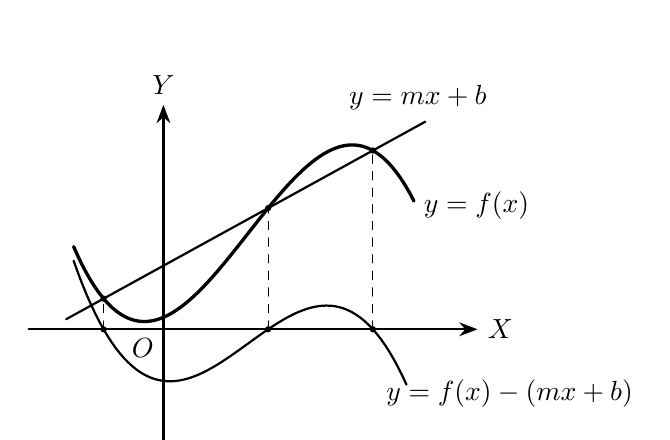
\begin{tikzpicture}[>=Stealth, scale=0.95, line cap=round, line join=round]
  \draw[->, thick] (-1.8, 0) -- (4.2, 0) node[right] {$X$};
  \draw[->, thick] (0, -1.6) -- (0, 3.0) node[above] {$Y$};
  \node[below left] at (0,0) {$O$};

  % Line y = mx + b: y = 0.55x + 0.85
  \draw[thick, domain=-1.3:3.5] plot (\x, {0.55*\x + 0.85});
  \node[above] at (3.4, 2.8) {$y=mx+b$};

  % Difference curve d(x) = -0.22*(x+0.8)*(x-1.4)*(x-2.8)
  % Intersects x-axis at x = -0.8, 1.4, 2.8
  \draw[thick, domain=-1.2:3.25, samples=80]
    plot (\x, {-0.22*(\x+0.8)*(\x-1.4)*(\x-2.8)});
  \node[below right] at (2.85, -0.55) {$y=f(x)-(mx+b)$};

  % Curve y = f(x) = mx + b + d(x)
  \draw[very thick, domain=-1.2:3.35, samples=80]
    plot (\x, {0.55*\x + 0.85 - 0.22*(\x+0.8)*(\x-1.4)*(\x-2.8)});
  \node[right] at (3.35, 1.65) {$y=f(x)$};

  % Vertical dashed lines at intersection x-coordinates
  \foreach \xi in {-0.8, 1.4, 2.8} {
    \draw[dashed] (\xi, 0) -- (\xi, {0.55*\xi + 0.85});
    \fill (\xi, 0) circle (1.2pt);
    \fill (\xi, {0.55*\xi + 0.85}) circle (1.2pt);
  }
\end{tikzpicture}
\end{figure}

解
\[ \begin{cases} y = f(x) \\ y = mx+b \end{cases} \]
即 $f(x) - mx - b = 0$ 此為 $n$ 次方程式，最多只有 $n$ 個根，故 $y=f(x)$ 與 $y=mx+b$ 最多交 $n$ 點。
\end{proof}\hfill$\#$

\begin{discussion}\label{disc:b6-2-3}
設實係數方程式 $f(x) = a_n x^n + a_{n-1} x^{n-1} + \dots + a_0, f(x)=0$ 無實根，而且 $a_n > 0$ 則對於任意 $x \in \mathbb{R}$，有 $f(x) \ge 0$。
\end{discussion}

\begin{proof}[【證明】]
$f(x) = a_n \{ x^2 - (\alpha_1+\bar{\alpha}_1)x + \alpha_1\bar{\alpha}_1 \} \dots \{ x^2 - (\alpha_r+\bar{\alpha}_r)x + \alpha_r\bar{\alpha}_r \}$。今觀察其中一個因式
\[ h_j(x) = x^2 - (\alpha_j+\bar{\alpha}_j)x + \alpha_j\bar{\alpha}_j \]
令 $\alpha_j = a_j + b_j i$ 則
\[ h_j(x) = x^2 - 2a_j x + a_j^2 + b_j^2 = (x-a_j)^2 + b_j^2 \]
如 $x$ 為實數，$(x-a_j)^2 + b_j^2 \ge 0$。因此對於 $x \in \mathbb{R}$，$f(x)$ 之各因式皆為 $\ge 0$。
\end{proof}\hfill$\#$

\begin{example}\label{ex:b6-2-5}
設 $f(x)=ax^2+bx+c=0$ 當 $b^2-4ac < 0$ 時，$ax^2+bx+c=0$ 無實根，故 $a f(x) \ge 0$。
\end{example}

\begin{proof}[【證】]
由配方法得
\[ f(x) = ax^2+bx+c = a \left[ \left(x+\dfrac{b}{2a}\right)^2 - \dfrac{b^2-4ac}{4a^2} \right] \]
$f(x)=0$ 無實根，則表示 $b^2-4ac < 0$，故 $f(x)$ 的值與 $a$ 的值同號。

\begin{figure}[H]
\centering
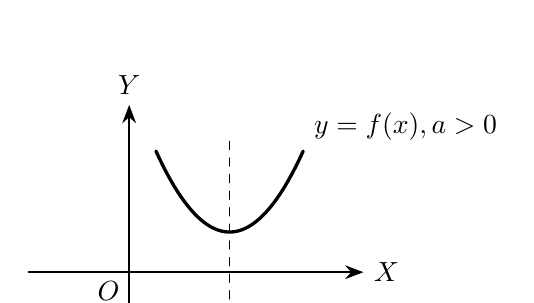
\begin{tikzpicture}[>=Stealth, scale=0.85, line cap=round, line join=round]
  \draw[->, thick] (-1.5, 0) -- (3.5, 0) node[right] {$X$};
  \draw[->, thick] (0, -0.6) -- (0, 2.5) node[above] {$Y$};
  \node[below left] at (0,0) {$O$};

  % Parabola completely above x-axis
  \draw[very thick, domain=0.4:2.6, samples=50] plot (\x, {(\x-1.5)^2 + 0.6}) node[above right] {$y=f(x), a>0$};
  \draw[dashed] (1.5, -0.4) -- (1.5, 2.0);
\end{tikzpicture}
\end{figure}
從幾何觀點說，$f(x)=0$ 無實根，即表示 $y=f(x)$ 的圖形與 $x$ 軸不相交，即拋物線不是在 $x$ 軸上方，便是在 $x$ 軸下方。
\end{proof}\hfill$\#$

\subsubsection*{作業 5}\label{hw:b6-2-5}
設一個 $2n$ 次方程式為
\[ f(x) = a_{2n} x^{2n} + a_{2(n-1)} x^{2(n-1)} + \dots + a_{2i} x^{2i} + \dots + a_2 x^2 + a_0 = 0 \]
如果 $f(x)=0$ 有一根為 $\alpha$，試證 $-\alpha$ 亦為其根。

\subsubsection*{丙、函數之圖示}\label{subsec:b6-2-2-c}

在三、四冊裡讀者已熟悉幾何與代數的轉換關係，如一次多項式函數可繪出直線，二次多項式函數可繪出拋物線等等。對於一個實係數多項式 $y=f(x)$，給定一實數 $x=a$，有一確定的對應值 $y=b=f(a)$，如此在 $xy$ 平面上就有一對應點 $(a, b)$。

\begin{figure}[H]
\centering
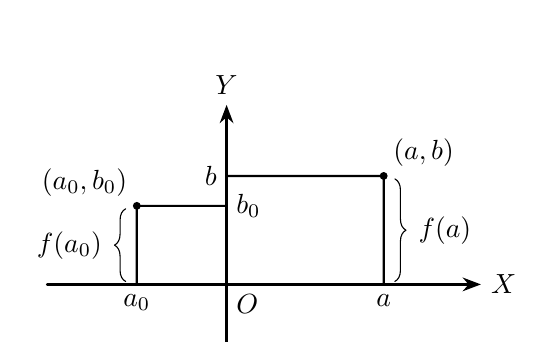
\begin{tikzpicture}[>=Stealth, scale=0.95, line cap=round, line join=round]
  \draw[->, thick] (-2.4, 0) -- (3.4, 0) node[right] {$X$};
  \draw[->, thick] (0, -0.9) -- (0, 2.4) node[above] {$Y$};
  \node[below right] at (0,0) {$O$};

  \coordinate (A0) at (-1.2, 1.05);
  \coordinate (A) at (2.1, 1.45);

  \draw[thick] (-1.2, 0) node[below] {$a_0$} -- (A0) -- (0, 1.05);
  \draw[thick] (2.1, 0) node[below] {$a$} -- (A) -- (0, 1.45);

  \fill (A0) circle (1.5pt) node[above left] {$(a_0, b_0)$};
  \fill (A) circle (1.5pt) node[above right] {$(a, b)$};
  \node[right] at (0, 1.05) {$b_0$};
  \node[left] at (0, 1.45) {$b$};

  % Braces matching original p.91
  \draw[decorate, decoration={brace, amplitude=4pt}] (-1.35, 0.04) -- (-1.35, 1.01) node[midway, left=5pt] {$f(a_0)$};
  \draw[decorate, decoration={brace, amplitude=4pt}] (2.25, 1.41) -- (2.25, 0.04) node[midway, right=5pt] {$f(a)$};
\end{tikzpicture}
\end{figure}

如果 $x$ 在 $X$ 軸上移動，就得到許多與之相對應的點，把這些點（圓滑地）描繪起來，稱為此函數之圖示。嚴格地說，我們必須描出當 $x$ 變動時所有的平面上的對應點的軌跡，才能確切地表出此函數之曲線。有時函數簡單，則不必那麼費事，如二點就可決定一直線。我們描述多項式亦可照著大略情形而繪的。

\begin{example}\label{ex:b6-2-6}
$y = x^3$
\end{example}

\begin{center}
\small
\renewcommand{\arraystretch}{1.2}
\begin{tabular}{|c|c|c|c|c|c|c|c|c|c|c|c|}
\hline
$x$ & $-5$ & $-4$ & $-3$ & $-2$ & $-1$ & $0$ & $1$ & $2$ & $3$ & $4$ & $5$ \\ \hline
$f(x)$ & $-125$ & $-64$ & $-27$ & $-8$ & $-1$ & $0$ & $1$ & $8$ & $27$ & $64$ & $125$ \\ \hline
\end{tabular}
\end{center}

\begin{figure}[H]
\centering
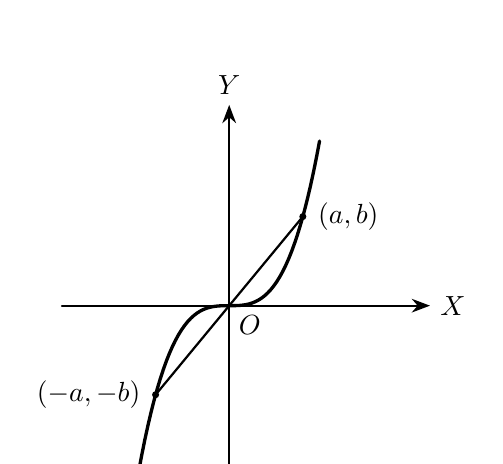
\begin{tikzpicture}[>=Stealth, scale=0.85, line cap=round, line join=round]
  \draw[->, thick] (-2.5, 0) -- (3.0, 0) node[right] {$X$};
  \draw[->, thick] (0, -2.5) -- (0, 3.0) node[above] {$Y$};
  \node[below right] at (0,0) {$O$};

  \draw[very thick, domain=-1.35:1.35, samples=60] plot (\x, {\x*\x*\x});
  % Symmetry secant line through origin (matching original p.91)
  \draw[thick] (-1.1, -1.331) -- (1.1, 1.331);
  \fill (1.1, 1.331) circle (1.5pt) node[right=2pt] {$(a, b)$};
  \fill (-1.1, -1.331) circle (1.5pt) node[left=2pt] {$(-a, -b)$};
\end{tikzpicture}
\end{figure}

繪圖時需要特別注意：
\begin{enumerate}[label=(\arabic*), leftmargin=2em]
  \item 對稱性
  \item 與 $X, Y$ 軸的交點（$X$ 截距，$Y$ 截距）
  \item 極大極小
  \item 曲線的升降
\end{enumerate}

\begin{example}\label{ex:b6-2-7}
$y = 2x^2 - x^4$
\end{example}

因為 $f(x)=f(-x)$，所以函數對於 $Y$ 軸對稱，我們只需討論 $x \ge 0$ 的情形：

\begin{center}
\small
\renewcommand{\arraystretch}{1.2}
\begin{tabular}{|c|c|c|c|c|c|c|}
\hline
$x$ & $0$ & $\dfrac{1}{2}$ & $1$ & $\sqrt{2}$ & $2$ & $3$ \\ \hline
$f(x)$ & $0$ & $\dfrac{7}{16}$ & $1$ & $0$ & $-8$ & $-63$ \\ \hline
\end{tabular}
\end{center}

$y = 1 - (1-2x^2+x^4) = 1 - (1-x^2)^2$，故此函數在 $x=1$ 取得最大值，$x \longrightarrow \infty$ 時 $f(x)$ 趨於負無窮大。

\begin{figure}[H]
\centering
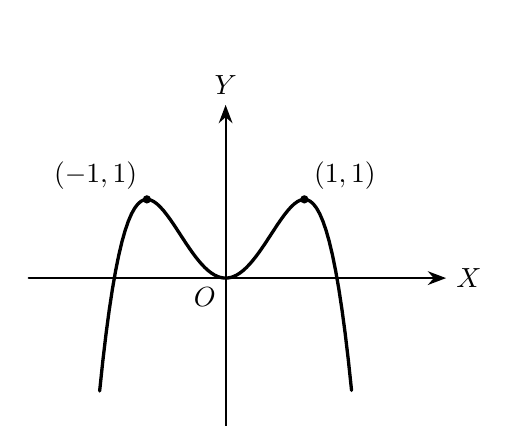
\begin{tikzpicture}[>=Stealth, scale=1.0, line cap=round, line join=round]
  \draw[->, thick] (-2.5, 0) -- (2.8, 0) node[right] {$X$};
  \draw[->, thick] (0, -2.0) -- (0, 2.2) node[above] {$Y$};
  \node[below left] at (0,0) {$O$};

  % M-curve: y = 2x^2 - x^4
  \draw[very thick, domain=-1.6:1.6, samples=80] plot (\x, {2*\x*\x - \x*\x*\x*\x});
  \fill (1, 1) circle (1.5pt) node[above right] {$(1, 1)$};
  \fill (-1, 1) circle (1.5pt) node[above left] {$(-1, 1)$};
\end{tikzpicture}
\end{figure}
\hfill$\#$

\subsubsection*{作業 6}\label{hw:b6-2-6}
試描繪下列各函數的曲線：
\begin{multicols}{2}
\begin{enumerate}[label=(\roman*)]
  \item $y = x^4$
  \item $y = x - x^3$
\end{enumerate}
\end{multicols}

\subsubsection*{習題 II-2}\label{sec:b6-ex2-2}

\begin{enumerate}[label=\arabic*., leftmargin=2em]
  \item 試求 $\sqrt{3-4i}$。
  \item 試解下列複數方程式：
  \begin{enumerate}[label=(\roman*)]
    \item $2z^4 - 2iz^3 + z^2 + 1 = 0$
    \item $z^3 + (1+i)z - (10+2i) = 0$
    \item $z^3 + (1+2i)z^2 - 3(1+2i)z + 1 + 4i = 0$
  \end{enumerate}
  \item 試作出一方程式以 $3, 2-i, 1+i$ 為根。
  \item 已知 $\omega = \dfrac{-1+\sqrt{3}i}{2}$ 為 $x^4+4x^3+8x^2+7x+4=0$ 的一根，試解方程式。
  \item 已知 $\sqrt{3}+\sqrt{2}i$ 為 $f(x)=0$ 的一根，試求最低次整係數方程式。
  \item 試解 $x^5+2x^4-3x^3-3x^2+2x+1=0$。
  \item 試分解 $f(x)=x^3+x^2+x+1$ 為一次或二次因式的乘積。
  \item 試分解 $f(x)=x^4-5x^3+4x^2-5x+1$ 為一次或二次因式的乘積。
  \item 試求出曲線 $y=x^3+4x+2$ 與直線 $y=x-2$ 的交點。
  \item 試解 $[x]^2+[x]-6=0$（$[x]$ 為高斯函數）。
  \item 若 $a, b, c$ 為正數，試證 $a^3+b^3+c^3 \ge 3abc$。
  \item 試證對於所有實數 $x$，$x^8+x^4+1 > 0$。
  \item 試繪出下列各函數的曲線：
  \begin{multicols}{2}
  \begin{enumerate}[label=(\roman*)]
    \item $y = 3 - 5x - x^2$
    \item $y = x^3 + 3x$
    \item $y = 2x^3 - 3x^2$
    \item $y = x^3 + x + 2$
    \item $y = x^4 - 4x$
    \item $y = x^4 - 2x^2$
    \item $y = x^4 - x^3$
    \item $y = x^4 - 2x + 1$
  \end{enumerate}
  \end{multicols}
\end{enumerate}

\subsection{根與係數的關係與對稱式}\label{sec:b6-2-3}
\resetsectcounters

\subsubsection*{甲、根與係數的關係}\label{subsec:b6-2-3-a}

在本書第一冊第七章裡有這樣一個定理：設 $\dfrac{b}{c}$ 是整係數方程式 $f(x) = a_n x^n + a_{n-1} x^{n-1} + \dots + a_0 = 0$ 的一個有理根，其中 $c > 0$，且 $(b, c)=1$ 則 $b$ 必定是 $a_0$ 的因數，$c$ 必定是 $a_n$ 的因數。上命題已指出一個有趣的事實：根與係數有密切的關係，特再舉一例來觀察：

設 $\beta_1, \beta_2, \beta_3$ 為方程式 $x^3 + a_1 x^2 + a_2 x + a_3 = 0$ 之三根，則有
\begin{align*}
x^3 + a_1 x^2 + a_2 x + a_3 &= (x-\beta_1)(x-\beta_2)(x-\beta_3) \\
&= x^3 - (\beta_1+\beta_2+\beta_3)x^2 + (\beta_1\beta_2+\beta_2\beta_3+\beta_3\beta_1)x - \beta_1\beta_2\beta_3
\end{align*}
比較兩邊係數得
\begin{align*}
a_1 &= -(\beta_1+\beta_2+\beta_3) \\
a_2 &= (\beta_1\beta_2+\beta_2\beta_3+\beta_3\beta_1) \\
a_3 &= -\beta_1\beta_2\beta_3
\end{align*}
更一般地觀察，令 $\beta_1, \beta_2, \dots, \beta_n$ 為方程式 $f(x) = x^n + a_1 x^{n-1} + a_2 x^{n-2} + \dots + a_{n-1} x + a_n = 0$ 之 $n$ 個根，則有
\[ f(x) = (x-\beta_1)(x-\beta_2)\dots(x-\beta_n) \]
展開右式後，比較兩端係數得
\begin{equation}
\begin{aligned}
a_1 &= -(\beta_1+\beta_2+\dots+\beta_n) = -(\text{所有根之和}) \\
a_2 &= \beta_1\beta_2+\beta_1\beta_3+\dots+\beta_1\beta_n+\beta_2\beta_3+\dots+\beta_{n-1}\beta_n = \text{所有根兩兩相乘所得之和} \\
a_3 &= -(\beta_1\beta_2\beta_3+\beta_1\beta_2\beta_4+\dots) = -(\text{所有根三三相乘所得之和}) \\
&\dots\dots\dots\dots \\
a_n &= (-1)^n \beta_1\beta_2\dots\beta_n = (-1)^n (\text{所有根之乘積})
\end{aligned} \tag{I} \label{eq:b6-2-3-I}
\end{equation}
若 $n$ 次方程式 $a_0 x^n + a_1 x^{n-1} + \dots + a_n = 0$ 的首項係數 $a_0 \ne 1$ 我們以 $a_0$ 遍除各項，再把方程式的缺項，以 0 補足，可以得到下述定理：

\begin{theorem}[根與係數的關係 / 韋達定理]\label{thm:b6-2-vieta}
設 $n$ 次方程式 $a_0 x^n + a_1 x^{n-1} + \dots + a_{n-1} x + a_n = 0$ 以 $\beta_1, \beta_2, \dots, \beta_n$ 為其根，則有
\begin{equation}
\begin{aligned}
\dfrac{a_1}{a_0} &= -(\beta_1+\dots+\beta_n) \\
\dfrac{a_2}{a_0} &= (\beta_1\beta_2+\dots+\beta_{n-1}\beta_n) \\
&\dots\dots\dots\dots \\
\dfrac{a_n}{a_0} &= (-1)^n \beta_1\beta_2\dots\beta_n
\end{aligned} \tag{II} \label{eq:b6-2-3-II}
\end{equation}
\end{theorem}

\begin{example}\label{ex:b6-2-8}
設 $x^3+7x^2-6x-72=0$ 有二根 3 與 $-4$，試求另一根。
\end{example}

\paragraph{【解】}
設 $3, -4, \beta$ 為此方程之三根，根據定理知
\[ 3(-4)\beta = (-1)^3(-72) = 72 \implies \beta = -6 \]\hfill$\#$

\begin{example}\label{ex:b6-2-9}
設方程式 $x^3+ax^2+bx+c=0$ 之三根成等比，試證 $b^3-a^3c=0$。
\end{example}

\paragraph{【解】}
設此方程式的三根為 $\dfrac{\alpha}{\beta}, \alpha, \alpha\beta$，則根據根與係數的關係得
\begin{align*}
\dfrac{\alpha}{\beta} + \alpha + \alpha\beta &= -a \\
\dfrac{\alpha^2}{\beta} + \alpha^2 + \alpha^2\beta &= b \\
\dfrac{\alpha}{\beta} \cdot \alpha \cdot \alpha\beta &= -c
\end{align*}
即
\begin{align}
\alpha\left(\dfrac{1}{\beta}+1+\beta\right) &= -a \label{eq:b6-2-3-ex2-1} \\
\alpha^2\left(\dfrac{1}{\beta}+1+\beta\right) &= b \label{eq:b6-2-3-ex2-2} \\
\alpha^3 &= -c \label{eq:b6-2-3-ex2-3}
\end{align}
$\dfrac{\eqref{eq:b6-2-3-ex2-2}}{\eqref{eq:b6-2-3-ex2-1}} \implies \alpha = -\dfrac{b}{a}$。代入 \eqref{eq:b6-2-3-ex2-3} 得 $-\dfrac{b^3}{a^3} = -c$，故 $b^3 - a^3 c = 0$。\hfill$\#$

\subsubsection*{作業 7}\label{hw:b6-2-7}
\begin{enumerate}[label=(\roman*), leftmargin=2em]
  \item 定義三階方陣 $\begin{pmatrix} a_{11} & a_{12} & a_{13} \\ a_{21} & a_{22} & a_{23} \\ a_{31} & a_{32} & a_{33} \end{pmatrix}$ 的特徵方程式為
  \[ \begin{vmatrix}
  a_{11}-x & a_{12} & a_{13} \\
  a_{21} & a_{22}-x & a_{23} \\
  a_{31} & a_{32} & a_{33}-x
  \end{vmatrix} = 0 \]
  試證此方程式諸根之和為 $(a_{11}+a_{22}+a_{33})$\phantomsection\label{note:b6-ch2-p95-trace}\footnote{【原書校訂】：原書此處印作「$-(a_{11}+a_{22}+a_{33})$」，漏消負號（$(-x)^3 + (a_{11}+a_{22}+a_{33})x^2 + \dots = 0 \implies$ 根之和為 $a_{11}+a_{22}+a_{33}$），茲予校訂正號。}，諸根之積為 $\begin{vmatrix} a_{11} & a_{12} & a_{13} \\ a_{21} & a_{22} & a_{23} \\ a_{31} & a_{32} & a_{33} \end{vmatrix}$。
  \item 推廣 (i) 至 $n$ 階方陣。
\end{enumerate}

\subsubsection*{作業 8}\label{hw:b6-2-8}
設方程式 $x^2+px+q=0$ 之二根為 $\alpha, \beta$，方程式 $x^2+Px+Q=0$ 之二根為 $\alpha(\alpha+1), \beta(\beta+1)$。試證
\[ P = p - p^2 + 2q, \qquad Q = q + q^2 - qp \]

\subsubsection*{*乙、對稱式基本定理}\label{subsec:b6-2-3-b}

對於上小段的 (I) 式，我們可以引用一種簡單的符號：
\begin{align*}
\beta_1+\beta_2+\dots+\beta_n &= \sum_{i=1}^n \beta_i \\
\beta_1\beta_2+\dots+\beta_{n-1}\beta_n &= \sum_{i=1, j=2, i<j}^n \beta_i \beta_j \\
\beta_1\beta_2\beta_3+\beta_1\beta_2\beta_4+\dots &= \sum_{1 \le i_1 < i_2 < i_3 \le n} \beta_{i_1}\beta_{i_2}\beta_{i_3}
\end{align*}
注意到：在這些式子中，把任意二數 $\beta_i, \beta_j$ 對調，所得的結果不變。又 $\beta_1^2+\beta_2^2+\dots+\beta_n^2$ 亦有這樣的性質。

\begin{definition}\label{def:b6-2-symmetric}
令 $P(x_1, \dots, x_n)$ 為一 $n$ 元多項式，如果在 $P(x_1, \dots, x_n)$ 中任意對調二不定元 $x_i, x_j$，所得的式子與原式相同，稱此多項式為\textbf{對稱多項式}或簡稱為\textbf{對稱式}。
\end{definition}

\begin{example}\label{ex:b6-2-10}
\begin{enumerate}[label=(\arabic*), leftmargin=2em]
  \item $x^3+y^3+z^3-3xyz$ \dots 三元齊次對稱式
  \item $x_1^2 x_2 + x_1^2 x_3 + x_2^2 x_1 + x_2^2 x_3 + x_3^2 x_1 + x_3^2 x_2$ \dots 三元齊次對稱式
  \item $x_1^4+x_2^4+x_3^4+x_4^4+x_1+x_2+x_3+x_4$ \dots 四元對稱式
\end{enumerate}
\end{example}

\begin{example}\label{ex:b6-2-11}
設方程式 $x^3+2x^2+7x+6=0$ 之三根為 $x_1, x_2, x_3$ 試求
\begin{multicols}{2}
\begin{enumerate}[label=(\roman*)]
  \item $x_1^2+x_2^2+x_3^2$
  \item $x_1^3+x_2^3+x_3^3$
\end{enumerate}
\end{multicols}
\end{example}

\paragraph{【解】}
\begin{enumerate}[label=(\roman*), leftmargin=2em]
  \item
  \begin{align*}
  x_1^2+x_2^2+x_3^2 &= (x_1+x_2+x_3)^2 - 2(x_1 x_2 + x_1 x_3 + x_2 x_3) \\
  &= (-2)^2 - 2 \cdot 7 = 4 - 14 = -10
  \end{align*}
  \item
  \begin{align*}
  x_1^3+x_2^3+x_3^3 &= x_1^3+x_2^3+x_3^3-3x_1 x_2 x_3 + 3x_1 x_2 x_3 \\
  &= (x_1+x_2+x_3)(x_1^2+x_2^2+x_3^2 - x_1 x_2 - x_1 x_3 - x_2 x_3) + 3x_1 x_2 x_3 \\
  &= (-2)(-10-7) + 3(-6) = 34 - 18 = 16
  \end{align*}
\end{enumerate}
\hfill$\#$

在上面例子中，我們將對稱多項式 (i), (ii) 表為某些簡單（或整齊些）的對稱多項式之有理式，而這些特別的對稱多項式，都是在 (I) 中出現的。是否任意對稱多項式都可以表成 (I) 中對稱多項式的有理式呢？這就是本節所要討論的。

設 $x_1, \dots, x_n$ 為不定元，令
\begin{equation}
\begin{aligned}
P_1 &= x_1 + \dots + x_n = \sum_{1 \le i \le n} x_i \\
P_2 &= x_1 x_2 + \dots + x_1 x_n + \dots + x_{n-1} x_n = \sum_{1 \le i < j \le n} x_i x_j \\
P_j &= \sum_{1 \le i_1 < i_2 < \dots < i_j \le n} x_{i_1}\dots x_{i_j} \\
&\dots\dots\dots\dots \\
P_n &= x_1 x_2 \dots x_n
\end{aligned} \tag{III} \label{eq:b6-2-3-III}
\end{equation}
這些多項式稱為 \textbf{$n$ 元基本對稱多項式}。

讀者注意到：
\begin{enumerate}[label=(\arabic*), leftmargin=2em]
  \item 0 是一個對稱式。
  \item 任意二 $n$ 元對稱式的和、差、積仍是對稱式。更一般地說：設 $f_1, f_2, \dots, f_t$ 為 $t$ 個對稱式，以這 $t$ 個式子為不定元的任一多項式 $P(f_1, f_2, \dots, f_t)$ 仍然是對稱式。特別地以 \eqref{eq:b6-2-3-III} 中的對稱式 $P_1, \dots, P_n$ 做出的任一多項式 $Q(P_1, \dots, P_n)$ 仍為對稱式。
  \item $P_1$ 是 $n$ 元一次式，$P_2$ 是二次式，\dots，$P_n$ 是 $n$ 次式。
  \item 令 $P_1', P_2', \dots, P_{n-1}'$ 是 $x_2, \dots, x_n$ 的 $n-1$ 元基本對稱式，則有
  \begin{equation}
  \begin{aligned}
  P_1 &= x_1 + x_2 + \dots + x_n = x_1 + P_1' \\
  P_2 &= x_1 x_2 + \dots + x_1 x_n + x_2 x_3 + \dots + x_{n-1} x_n = x_1 P_1' + P_2' \\
  P_i &= x_1 P_{i-1}' + P_i' \qquad i=2, \dots, n-1 \\
  &\dots\dots\dots\dots \\
  P_n &= x_1 P_{n-1}'
  \end{aligned} \tag{IV} \label{eq:b6-2-3-IV}
  \end{equation}
  \item 下列等式成立：
  \begin{equation}
  x_1^n - P_1 x_1^{n-1} + P_2 x_1^{n-2} + \dots + (-1)^n P_n = 0 \tag{V} \label{eq:b6-2-3-V}
  \end{equation}
\end{enumerate}

\begin{proof}[【證明】]
考慮一函數 $f(z) = (z-x_1)(z-x_2)\dots(z-x_n) = z^n - P_1 z^{n-1} + P_2 z^{n-2} + \dots + (-1)^n P_n$。因為 $f(x_1)=0$，故得上式。
\end{proof}

\begin{lemma}\label{lem:b6-2-sym-vandermonde}
設 $b_0, b_1, \dots, b_{n-1}$ 是 $n$ 元 $(x_1, \dots, x_n)$ 對稱多項式，而且有下列等式關係：
\begin{equation}
b_0 x_1^{n-1} + b_1 x_1^{n-2} + \dots + b_{n-2} x_1 + b_{n-1} = 0 \tag{VI} \label{eq:b6-2-3-VI}
\end{equation}
則
\[ b_0 = b_1 = \dots = b_{n-1} = 0 \]
\end{lemma}

\begin{proof}[【證明】]
在 \eqref{eq:b6-2-3-VI} 式左邊中將所有 $x_1$ 以 $x_2$ 代換，因 $b_0, \dots, b_{n-1}$ 為對稱式所以不變，得
\[ b_0 x_2^{n-1} + b_1 x_2^{n-2} + \dots + b_{n-2} x_2 + b_{n-1} = 0 \]
同理 \eqref{eq:b6-2-3-VI} 式分別以 $x_3, \dots, x_n$ 代替 $x_1$ 恆等式仍然成立而得下列方程式組：
\[ \begin{cases}
b_0 x_1^{n-1} + \dots + b_{n-1} = 0 \\
b_0 x_2^{n-1} + \dots + b_{n-1} = 0 \\
\dots\dots\dots\dots \\
b_0 x_n^{n-1} + \dots + b_{n-1} = 0
\end{cases} \]
此方程式組為關於 $b_0, \dots, b_{n-1}$ 的一次聯立方程式，因為係數行列式（此係為 Vandermonde 行列式）：
\[ \begin{vmatrix}
x_1^{n-1} & x_1^{n-2} & \dots & 1 \\
x_2^{n-1} & x_2^{n-2} & \dots & 1 \\
\vdots & \vdots & & \vdots \\
x_n^{n-1} & x_n^{n-2} & \dots & 1
\end{vmatrix} = \pm \prod_{i<j}^n (x_i-x_j) \ne 0 \]
根據克萊瑪法則，其解為
\[ b_0 = b_1 = \dots = b_{n-1} = 0 \]
故得證。\end{proof}\hfill$\#$

利用上面五個特性與補助定理，我們可以用減少不定元的個數與降低次數的方法把所有的對稱式表為基本對稱式之多項式：

設 $P=P(x_1, \dots, x_n)$ 為 $n$ 元對稱式。
\begin{enumerate}[label=(\Roman*), leftmargin=2em]
  \item 把 $P$ 看為 $x_2, \dots, x_n$ 的 $n-1$ 元對稱式，而化解為 $P_1', P_2', \dots, P_{n-1}'$ 的多項式：
  \[ P(x_1, \dots, x_n) = g(x_1, P_1', P_2', \dots, P_{n-1}') \]
  \item 利用 \eqref{eq:b6-2-3-IV} 消去 $P_1', P_2', \dots, P_{n-1}'$ 得一以 $x_1, P_1, P_2, \dots, P_n$ 為元的多項式：
  \[ P(x_1, \dots, x_n) = g(x_1, P_1', \dots, P_{n-1}') = h(x_1, P_1, P_2, \dots, P_n) \]
  \item 把 $h(x_1, P_1, P_2, \dots, P_n)$ 寫成 $x_1$ 的降冪多項式：
  \[ h = B_0 x_1^k + B_1 x_1^{k-1} + \dots + B_k \]
  （其中當然 $B_i$ 為 $P_1, \dots, P_n$ 的合成，故為對稱式）
  \item 
  \begin{enumerate}[label=(\alph*)]
    \item 如果 $k \le n-1$，因為
    \[ B_0 x_1^k + B_1 x_1^{k-1} + \dots + B_k - P = 0 \]
    各項為對稱式，利用補助定理得 $P = B_k$。
    \item 如果 $k > n-1$，利用 \eqref{eq:b6-2-3-V}
    \[ x_1^n = P_1 x_1^{n-1} - P_2 x_1^{n-2} + \dots - (-1)^n P_n \]
    代入 $h$，可以降低 $x_1$ 的次數至 $n-1$，得
    \[ P(x_1, \dots, x_n) = b_0 x_1^t + b_1 x_1^{t-1} + \dots + b_t, \quad t \le n-1 \]
    故 $P(x_1, \dots, x_n) = b_t$。
  \end{enumerate}
\end{enumerate}
這裡 $B_k, b_t$ 都是 $P_1, \dots, P_n$ 的多項式。由上面四個步驟得：

\begin{theorem}[對稱式基本定理]\label{thm:b6-2-fundamental-symmetric}
每一個對稱多項式皆可表為基本對稱式之多項式。
\end{theorem}

\begin{example}\label{ex:b6-2-12}
試把 $x^3+y^3+z^3+w^3$ 表為四元基本對稱式的多項式。
\end{example}

\paragraph{【解】}
令
\[ \begin{cases}
P_1 = x+y+z+w \\
P_2 = xy+xz+xw+yz+yw+zw \\
P_3 = xyz+xyw+xzw+yzw \\
P_4 = xyzw
\end{cases} \]
為四元基本對稱式。令
\[ \begin{cases}
P_1' = y+z+w \\
P_2' = yz+yw+zw \\
P_3' = yzw
\end{cases} \]
為 $y, z, w$ 三元基本對稱式。已知（〔例 4〕）
\begin{align*}
y^2+z^2+w^2 &= (y+z+w)^2 - 2(yz+yw+zw) = P_1'^2 - 2P_2' \\
y^3+z^3+w^3 &= (y+z+w)(y^2+z^2+w^2-yz-yw-zw) + 3yzw \\
&= P_1'(P_1'^2 - 3P_2') + 3P_3'
\end{align*}
\begin{enumerate}[label=(\Roman*), leftmargin=2em]
  \item 現令 $x$ 為常數，則
  \begin{equation}
  x^3+y^3+z^3+w^3 = x^3 + P_1'(P_1'^2 - 3P_2') + 3P_3' \label{eq:b6-2-3-ex5-1}
  \end{equation}
  \item 從 \eqref{eq:b6-2-3-IV} 得
  \begin{align*}
  P_1' &= P_1 - x \\
  P_2' &= P_2 - x P_1' = P_2 - x P_1 + x^2 \\
  P_3' &= P_3 - x P_2' = P_3 - x P_2 + x^2 P_1 - x^3
  \end{align*}
  代入 \eqref{eq:b6-2-3-ex5-1}：
  \begin{align*}
  P &= x^3+y^3+z^3+w^3 = x^3 + (P_1-x)[(P_1-x)^2 - 3(P_2 - x P_1 + x^2)] \\
  &\quad + 3(P_3 - x P_2 + x^2 P_1 - x^3)
  \end{align*}
  整理之，得
  \item $b_0 x^3 + b_1 x^2 + b_2 x + P_1^3 - 3P_1 P_2 + 3P_3 - P = 0$。\\
  因係數皆為四元對稱式，根據補助定理得
  \item $x^3+y^3+z^3+w^3 = P = P_1^3 - 3P_1 P_2 + 3P_3$。
\end{enumerate}
\hfill$\#$

\begin{example}\label{ex:b6-2-13}
試把 $x^3+y^3+z^3$ 表為三元基本對稱式之多項式。
\end{example}

\paragraph{【解】}
令
\[ \begin{cases}
P_1 = x+y+z \\
P_2 = xy+xz+yz \\
P_3 = xyz
\end{cases} \qquad \begin{cases}
P_1' = y+z \\
P_2' = yz
\end{cases} \]
又知
\begin{align*}
y^3+z^3 &= y^3+z^3+3y^2z+3yz^2 - 3yz(y+z) \\
&= (y+z)^3 - 3yz(y+z) = P_1'^3 - 3P_2'P_1'
\end{align*}
令 $x$ 為常數，則
\begin{enumerate}[label=(\Roman*), leftmargin=2em]
  \item $P = x^3+y^3+z^3 = x^3 + P_1'^3 - 3P_2'P_1'$
  \item $= x^3 + (P_1-x)^3 - 3(P_2 - x P_1 + x^2)(P_1-x) = 3x^3 - 3P_1 x^2 + 3P_2 x + P_1^3 - 3P_1 P_2$
  \item 得 $3x^3 - 3P_1 x^2 + 3P_2 x + P_1^3 - 3P_1 P_2 - P = 0$
  \item 由 \eqref{eq:b6-2-3-V} 式知 $x^3 - P_1 x^2 + P_2 x - P_3 = 0$，故 $x^3 = P_1 x^2 - P_2 x + P_3$ 代入得
  \[ 3(P_1 x^2 - P_2 x + P_3) - 3P_1 x^2 + 3P_2 x + P_1^3 - 3P_1 P_2 - P = 0 \]
  即
  \[ b_0 x^2 + b_1 x + P_1^3 - 3P_1 P_2 + 3P_3 - P = 0 \]
  其中的係數皆為三元對稱式，今由補助定理知
  \[ x^3+y^3+z^3 = P = P_1^3 - 3P_1 P_2 + 3P_3 \]
\end{enumerate}
\hfill$\#$

\subsubsection*{作業 9}\label{hw:b6-2-9}
試把下列對稱式表為基本對稱式之多項式：
\begin{enumerate}[label=(\roman*)]
  \item $x_1^4 + x_2^4 + x_3^4$
  \item $x_1^2 x_2 + x_1^2 x_3 + x_2^2 x_1 + x_2^2 x_3 + x_3^2 x_1 + x_3^2 x_2$
  \item $x_1^4 + x_2^4 + x_1^3 + x_2^3$
\end{enumerate}

\subsubsection*{習題 II-3}\label{sec:b6-ex2-3}

\begin{enumerate}[label=\arabic*., leftmargin=2em]
  \item 已知方程式 $2x^3+3x^2-23x-12=0$ 有一根為 3，求其他二根。
  \item 設方程式 $x^3-3\sqrt{2}x^2-12x+16\sqrt{2}=0$ 的三根成等差級數，求三根。
  \item 已知 $14x^3-13x^2-18x+9=0$ 的三根成調和級數，試解之。
  \item 試作方程式使其根為 $x^3+px^2+qx+r=0$ 的根的 (i) 平方 (ii) 立方。
  \item $\alpha, \beta, \gamma$ 為方程式 $x^3+px^2+qx+r=0$ 的三根，試作一方程式使其三根為：
  \begin{enumerate}[label=(\roman*)]
    \item $\alpha+\beta, \beta+\gamma, \gamma+\alpha$
    \item $\dfrac{\beta+\gamma-\alpha}{2}, \dfrac{\gamma+\alpha-\beta}{2}, \dfrac{\alpha+\beta-\gamma}{2}$
    \item $\beta^2+\beta\gamma+\gamma^2, \gamma^2+\gamma\alpha+\alpha^2, \alpha^2+\alpha\beta+\beta^2$
    \item $\alpha - \dfrac{1}{\beta\gamma}, \beta - \dfrac{1}{\gamma\alpha}, \gamma - \dfrac{1}{\alpha\beta}$
    \item $\dfrac{\alpha}{\beta+\gamma}, \dfrac{\beta}{\gamma+\alpha}, \dfrac{\gamma}{\alpha+\beta}$
  \end{enumerate}
  \item 三階方陣 $(a_{ij})$ 的特徵方程式的三根為 $\alpha, \beta, \gamma$，試求 $\alpha\beta+\beta\gamma+\gamma\alpha$ 的值。
  \item 把下列對稱式表為基本對稱式的多項式：
  \begin{enumerate}[label=(\roman*)]
    \item $(x_1+x_2+x_3)^3 - (-x_1+x_2+x_3)^3 - (x_1-x_2+x_3)^3 - (x_1+x_2-x_3)^3$
    \item $x_1^2 x_2^2 + x_2^2 x_3^2 + x_3^2 x_1^2 + x_1^2 x_3^2 + x_1^2 x_4^2 + x_2^2 x_4^2$
    \item $\sum_{1 \le i, j, k \le 4} x_i^2 x_j x_k$
  \end{enumerate}
  \item 令 $P_i$ 為 $x_1, \dots, x_n$ 的基本對稱式，$S_k = \sum_{i=1}^n x_i^k, k=1, 2, 3, \dots$ 試證
  \[ S_k - P_1 S_{k-1} + P_2 S_{k-2} + \dots + (-1)^n P_n S_{k-n} = 0 \]
  \item 四次方程式 $x^4+px^3+qx^2+rx+t=0$ 的二根乘積等於另二根乘積，其充要條件如何？
\end{enumerate}

\subsection{多項式函數的導數}\label{sec:b6-2-4}
\resetsectcounters

一般函數的導數的討論是微分學裡的主題，本節只處理實係數多項式函數。

\subsubsection*{甲、導函數}\label{subsec:b6-2-4-a}

現在先來觀察一例。令 $f(x)=5x^2+2x+7$ 以 $x+h$ 代 $x$ 然後按 $h$ 的升冪排列之：
\begin{align*}
f(x+h) &= 5(x+h)^2 + 2(x+h) + 7 \\
&= 5(x^2+2xh+h^2) + 2(x+h) + 7 \\
&= (5x^2+2x+7) + (10x+2)h + 5h^2
\end{align*}
我們看出不含 $h$ 的項為原函數。至於 $h$ 的一次項，二次項的係數是什麼？能否簡單的求得？這就是本節裡要加以討論的問題。

\begin{definition}\label{def:b6-2-derivative}
設多項式函數為 $f(x)=a_n x^n + a_{n-1} x^{n-1} + \dots + a_0$，在 $f(x)$ 中以 $x+h$ 代 $x$，再展開為 $h$ 的升冪多項式得
\begin{equation}
f(x+h) = a_n(x+h)^n + a_{n-1}(x+h)^{n-1} + \dots + a_0 = f(x) + f_1(x)h + f_2(x)h^2 + \dots + f_n(x)h^n \label{eq:b6-2-4-1}
\end{equation}
$h$ 的係數 $f_1(x)$ 稱為 $f(x)$ 的\textbf{第一階導函數}（簡稱\textbf{導函數}）通常以 $f'(x)$ 表示之。
\end{definition}

\paragraph{注意：}$f(x)$ 的導函數 $f'(x)$ 仍為 $x$ 的函數。導函數 $f'(x)$ 在 $x=\alpha$ 的值，$f'(\alpha)$，稱為函數 $f(x)$ 在 $x=\alpha$ 的\textbf{導數}。

\begin{discussion}\label{disc:b6-2-4}
從 (1) 式中得
\[ f(x+h) - f(x) = f'(x)h + f_2(x)h^2 + \dots + f_n(x)h^n \]
故
\[ \dfrac{f(x+h)-f(x)}{h} = f'(x) + f_2(x)h + \dots + f_n(x)h^{n-1} \]
當所取的 $h$ 很小且趨近於 0，上式右邊趨近於 $f'(x)$，這一現象，可用下式表示：
\[ \lim_{h \to 0} \dfrac{f(x+h)-f(x)}{h} = f'(x) \]
\end{discussion}

\begin{theorem}\label{thm:b6-2-diff-rules}
設 $f(x), g(x)$ 為二多項式函數，則
\begin{enumerate}[label=(\arabic*), leftmargin=2em]
  \item $(f(x)+g(x))' = f'(x) + g'(x)$
  \item $(f(x)g(x))' = f'(x)g(x) + f(x)g'(x)$
\end{enumerate}
\end{theorem}

\begin{proof}[【證明】]
設
\begin{align}
f(x+h) &= f(x) + f'(x)h + f_2(x)h^2 + \dots + f_n(x)h^n \label{eq:b6-2-4-p1} \\
g(x+h) &= g(x) + g'(x)h + g_2(x)h^2 + \dots + g_n(x)h^n \label{eq:b6-2-4-p2}
\end{align}
由 \eqref{eq:b6-2-4-p1} 式乘 \eqref{eq:b6-2-4-p2} 式及 \eqref{eq:b6-2-4-p1} 式加 \eqref{eq:b6-2-4-p2} 式得
\begin{align*}
f(x+h)g(x+h) &= f(x)g(x) + (f'(x)g(x) + g'(x)f(x))h \\
&\quad + (f(x)g_2(x) + f'(x)g'(x) + g(x)f_2(x))h^2 + \dots \\
f(x+h)+g(x+h) &= f(x)+g(x) + (f'(x)+g'(x))h + (f_2(x)+g_2(x))h^2 + \dots
\end{align*}
觀察 $h$ 的係數我們證出
\begin{align*}
(f(x)+g(x))' &= f'(x) + g'(x) \\
(f(x)g(x))' &= f'(x)g(x) + f(x)g'(x)
\end{align*}
\end{proof}\hfill$\#$

\begin{corollary}\label{cor:b6-2-diff-multi}
設 $f_1(x), \dots, f_n(x)$ 為 $n$ 個多項式函數，則
\begin{enumerate}[label=(\arabic*), leftmargin=2em]
  \item $(f_1(x)+\dots+f_n(x))' = f_1'(x) + \dots + f_n'(x)$
  \item $(f_1(x)f_2(x)\dots f_n(x))' = f_1'(x)f_2(x)\dots f_n(x) + f_1(x)f_2'(x)f_3(x)\dots f_n(x)$ \\
  $\phantom{(f_1(x)f_2(x)\dots f_n(x))' ={}} + \dots + f_1(x)f_2(x)\dots f_n'(x)$
\end{enumerate}
\end{corollary}

\begin{proof}[【證明】]
利用數學歸納法。
\end{proof}\hfill$\#$

\begin{example}\label{ex:b6-2-14}
試求 $f(x)=a$ 的導函數。
\end{example}

\paragraph{【解】}
$f(x+h)=a$，故 $f'(x)=0$。\hfill$\#$

\begin{example}\label{ex:b6-2-15}
試求 $f(x)=ax^n$ 的導函數 ($n \ge 1$)。
\end{example}

\paragraph{【解】}
$f(x+h) = a(x+h)^n = ax^n + anx^{n-1}h + a\binom{n}{2}x^{n-2}h^2 + \dots + ah^n$，故
\[ f'(x) = anx^{n-1} \]\hfill$\#$

\begin{corollary}\label{cor:b6-2-poly-diff}
令多項式為 $f(x) = a_n x^n + a_{n-1} x^{n-1} + \dots + a_1 x + a_0$，則
\[ f'(x) = n a_n x^{n-1} + (n-1)a_{n-1} x^{n-2} + \dots + a_1 \]
\end{corollary}

\begin{proof}[【證明】]
利用推論 1 與例 1, 2。
\end{proof}\hfill$\#$

\begin{example}\label{ex:b6-2-16}
$((x+7)(3x^3+6x+7))'$
\end{example}

\paragraph{【解】}
\begin{align*}
((x+7)(3x^3+6x+7))' &= (x+7)'(3x^3+6x+7) + (3x^3+6x+7)'(x+7) \\
&= 3x^3+6x+7 + (9x^2+6)(x+7) \\
&= 3x^3+6x+7 + 9x^3+6x+63x^2+42 \\
&= 12x^3+63x^2+12x+49
\end{align*}
\hfill$\#$

我們稱 $f'(x)$ 的導函數為 $f(x)$ 的\textbf{第二階導函數}，而記為 $f''(x)$。仿此，$f(x)$ 的第三階、第四階、\dots 第 $n$ 階導函數皆可同樣定義，記為 $f'''(x), f^{(4)}(x), \dots, f^{(n)}(x)$。

\begin{example}\label{ex:b6-2-17}
令 $f(x)=x^4+2x^3+7x+2$，求 $f'(0), f''(0), f'''(0)$。
\end{example}

\paragraph{【解】}
\begin{align*}
f'(x) &= 4x^3+6x^2+7 &\implies f'(0) &= 4 \cdot 0^3 + 6 \cdot 0^2 + 7 = 7 \\
f''(x) &= 12x^2+12x &\implies f''(0) &= 12 \cdot 0^2 + 12 \cdot 0 = 0 \\
f'''(x) &= 24x+12 &\implies f'''(0) &= 12
\end{align*}
\hfill$\#$

\subsubsection*{作業 10}\label{hw:b6-2-10}
\begin{enumerate}[label=(\roman*), leftmargin=2em]
  \item 令 $f(x)=(x+8)(x^4+x^3+2x^2+7)$ 試求 $f'(1), f''(0), f'''(-1), f^{(4)}(0)$。
  \item 試按定義推求 $f(x)=ax^n$ 的第二、第三階導函數。
  \item 設 $f(x)=a_n x^n + a_{n-1} x^{n-1} + \dots + a_0$，試證 $f^{(n+1)}(x) = 0$。
  \item 試證 $f(x)$ 的第二（第三）階導函數為 $f(x+h)$ 以 $h$ 展開的 $h^2(h^3)$ 項的 $2!(3!)$ 倍。
\end{enumerate}

\subsubsection*{乙、重根定理}\label{subsec:b6-2-4-b}

一多項式 $f(x)$ 能被 $(x-\alpha)^k$ 整除，而不能被 $(x-\alpha)^{k+1}$ 整除，我們稱 $\alpha$ 是 $f(x)=0$ 的 \textbf{$k$ 重根}。

\begin{theorem}[重根定理]\label{thm:b6-2-multiple-root}
若 $\alpha$ 為 $n$ 次方程式 $f(x)=0$ 之 $k$ 重根，則 $\alpha$ 為 $f'(x)=0$ 的 $k-1$ 重根。
\end{theorem}

\begin{proof}[【證明】]
因 $f(x)=0$ 有 $k$ 重根 $\alpha$，故
\[ f(x) = (x-\alpha)^k g(x), \qquad (x-\alpha) \nmid g(x) \]
兩端取導數，得
\begin{align*}
f'(x) &= ((x-\alpha)^k)' g(x) + (x-\alpha)^k g'(x) \\
&= k(x-\alpha)^{k-1} g(x) + (x-\alpha)^k g'(x)
\end{align*}
知 $(x-\alpha)^{k-1} \mid f'(x)$。若 $f'(x)$ 能被 $(x-\alpha)^k$ 整除，則
\begin{align*}
(x-\alpha)^k &\mid [f'(x) - (x-\alpha)^k g'(x)] = k(x-\alpha)^{k-1} g(x) \\
\implies (x-\alpha) &\mid g(x)
\end{align*}
此為矛盾，所以 $\alpha$ 為 $f'(x)$ 的 $k-1$ 重根。
\end{proof}\hfill$\#$

\begin{corollary}\label{cor:b6-2-gcd-root}
若 $f(x)=0$ 有 $k$ 重根 $\alpha$，則 $f(x)$ 與 $f'(x)$ 有公因式 $(x-\alpha)^{k-1}$。
\end{corollary}

\begin{example}\label{ex:b6-2-18}
設 1 為 $x^3+px^2+7x+q=0$ 的二重根，試求 $p, q$ 之值。
\end{example}

\paragraph{【解】}
1 為 $x^3+px^2+7x+q=0$ 之一根，故
\begin{equation}
1 + p + 7 + q = 0 \label{eq:b6-2-4-ex5-1}
\end{equation}
由定理知 1 亦為 $3x^2+2px+7=0$ 之一根，故
\begin{equation}
3 + 2p + 7 = 0 \label{eq:b6-2-4-ex5-2}
\end{equation}
從 \eqref{eq:b6-2-4-ex5-1}, \eqref{eq:b6-2-4-ex5-2} 解 $p, q$ 得
\[ \begin{cases} p = -5 \\ q = -3 \end{cases} \]\hfill$\#$

\subsubsection*{作業 11}\label{hw:b6-2-11}
\begin{enumerate}[label=(\roman*), leftmargin=2em]
  \item 若 2 為 $x^4-5mx^2+7x+4n=0$ 之二重根，試求 $m, n$。
  \item 試證 $x^n-a^n$ 無重根 ($a \ne 0$)。
\end{enumerate}

\subsubsection*{丙、泰勒展開式 (Taylor's Expansion)}\label{subsec:b6-2-4-c}

令 $f(x)=a_m x^m, g(x)=a_n x^n, \quad n=m+k$。利用二項式定理展開 $f(x+h), g(x+h)$ 得
\begin{align*}
f(x+h) &= a_m(x+h)^m = a_m x^m + m a_m x^{m-1}h + m(m-1)a_m x^{m-2}\dfrac{h^2}{2!} \\
&\quad + m(m-1)(m-2)a_m x^{m-3}\dfrac{h^3}{3!} + \dots + a_m m(m-1)\dots(m-m+1)\dfrac{h^m}{m!} \\
&\quad + 0 + \dots + 0 \cdot \dfrac{h^n}{n!} \\
g(x+h) &= a_n x^n + n a_n x^{n-1}h + n(n-1)a_n x^{n-2}\dfrac{h^2}{2!} + n(n-1)(n-2)a_n x^{n-3}\dfrac{h^3}{3!} \\
&\quad + \dots + a_n n(n-1)\dots(n-m+1)x^{n-m}\dfrac{h^m}{m!} \\
&\quad + \dots + n(n-1)\dots(n-n+1)a_n \dfrac{h^n}{n!}
\end{align*}
觀察 $h^i$ 的係數知：
$2!$ 倍 $h^2$ 的係數 $m(m-1)a_m x^{m-2}$，恰為 $f(x)$ 之二階導函數；
$3!$ 倍 $h^3$ 的係數 $m(m-1)(m-2)a_m x^{m-3}$，恰為 $f(x)$ 之三階導函數；
一般說來，$i!$ 倍 $h^i$ 的係數 $m(m-1)\dots(m-i+1)a_m x^{m-i}$，恰為 $f(x)$ 之 $i$ 階導函數。
所以展開式 $f(x+h)$ 可表成：
\begin{align}
f(x+h) &= f(x) + f'(x)h + f''(x)\dfrac{h^2}{2!} + f'''(x)\dfrac{h^3}{3!} + \dots + f^{(m)}(x)\dfrac{h^m}{m!} \label{eq:b6-2-4-taylor-f} \\
g(x+h) &= g(x) + g'(x)h + g''(x)\dfrac{h^2}{2!} + \dots + g^{(m)}(x)\dfrac{h^m}{m!} + \dots + g^{(n)}(x)\dfrac{h^n}{n!} \label{eq:b6-2-4-taylor-g}
\end{align}
因為 $f^{(m+1)}(x), f^{(m+2)}(x), \dots, f^{(n)}(x)$ 皆為 0，我們可以延長 \eqref{eq:b6-2-4-taylor-f} 式而寫成
\begin{align}
f(x+h) &= f(x) + f'(x)h + \dots + f^{(m)}(x)\dfrac{h^m}{m!} + f^{(m+1)}(x)\dfrac{h^{m+1}}{(m+1)!} + \dots + f^{(n)}(x)\dfrac{h^n}{n!} \label{eq:b6-2-4-taylor-fp}
\end{align}
令 $P(x)=f(x)+g(x)$，因 $P'(x)=f'(x)+g'(x), \dots, P^{(i)}(x)=f^{(i)}(x)+g^{(i)}(x)$，\eqref{eq:b6-2-4-taylor-f}+\eqref{eq:b6-2-4-taylor-g} 得
\[ P(x+h) = a_m(x+h)^m + a_n(x+h)^n = P(x) + P'(x)h + P''(x)\dfrac{h^2}{2!} + \dots + P^{(n)}(x)\dfrac{h^n}{n!} \]
推廣之，令 $g_0(x)=a_0, g_1(x)=a_1 x, g_2(x)=a_2 x^2, \dots, g_n(x)=a_n x^n$，
$f(x) = g_n(x) + \dots + g_0(x) = a_n x^n + a_{n-1} x^{n-1} + \dots + a_0$。

\begin{theorem}[Taylor's 展開式]\label{thm:b6-2-taylor}
令 $n$ 次多項式為 $f(x)=a_n x^n + a_{n-1} x^{n-1} + \dots + a_0$，展開 $f(x+h)$ 則
\begin{equation}
f(x+h) = f(x) + f'(x)h + f''(x)\dfrac{h^2}{2!} + \dots + f^{(n)}(x)\dfrac{h^n}{n!} \tag{I} \label{eq:b6-2-4-taylor-I}
\end{equation}
\end{theorem}

上面 (I) 式稱為 $f(x+h)$ 的泰勒展開式。

\begin{example}\label{ex:b6-2-19}
設函數為 $f(x)=x^3+x^2+x+1$ 試求 $f(x+h)$ 的泰勒展開式。
\end{example}

\paragraph{【解】}
\begin{align*}
f(x+h) &= (x+h)^3 + (x+h)^2 + (x+h) + 1 \\
&= x^3+3x^2h+3xh^2+h^3 + x^2+2xh+h^2 + x+h + 1 \\
&= (x^3+x^2+x+1) + (3x^2+2x+1)h + (3x+1)h^2 + h^3 \\
&= f(x) + f'(x)h + f''(x)\dfrac{h^2}{2!} + f'''(x)\dfrac{h^3}{3!}
\end{align*}
\hfill$\#$

\subsubsection*{作業 12}\label{hw:b6-2-12}
設函數 $f(x)=x^7+x^6+x^5$，試求 $f(x+h)$ 的泰勒展開式。

在 (I) 中，我們做些代換，可以寫成其他形式。令 $x=a+(x-a)$ 得
\begin{equation}
f(x) = f(a+(x-a)) = f(a) + f'(a)(x-a) + f''(a)\dfrac{(x-a)^2}{2!} + \dots + f^{(n)}(a)\dfrac{(x-a)^n}{n!} \tag{II} \label{eq:b6-2-4-taylor-II}
\end{equation}
此稱為 $f(x)$ 在 $x=a$ 點的泰勒展開式。

\begin{example}\label{ex:b6-2-20}
設 $f(x)=x^3-x^2-1$ 得 $f(1)=-1, f'(1)=1, f''(1)=4, f'''(1)=6$。
\end{example}

\paragraph{【解】}
\begin{align*}
f(x) &= f(1+(x-1)) = f(1) + f'(1)(x-1) + f''(1)\dfrac{(x-1)^2}{2!} + f'''(1)\dfrac{(x-1)^3}{3!} \\
&= -1 + (x-1) + 4\dfrac{(x-1)^2}{2!} + 6\dfrac{(x-1)^3}{3!} \\
&= -1 + (x-1) + 2(x-1)^2 + (x-1)^3
\end{align*}
\hfill$\#$

上例告訴我們多項式可以變換為 $(x-a)$ 的升冪展開式。這樣的變換，通稱為\textbf{平行變換}。多項式的變形我們第一冊已利用綜合除法做過。泰勒展開式特別指出展開式係數與導函數的關係。利用泰勒展開式將多項式變形，可用於求多項式函數在某點的近似值。

\begin{example}\label{ex:b6-2-21}
設 $f(x)=x^5+2x^2-3x-1$ 求 $f(2.003)$ 之近似值準確至小數點以下第三位。
\end{example}

\paragraph{【解】}
\begin{align*}
f'(x) &= 5x^4+4x-3, & f''(x) &= 20x^3+4, & f'''(x) &= 60x^2, \\
f^{(4)}(x) &= 120x, & f^{(5)}(x) &= 120 \\
f'(2) &= 85, & f''(2) &= 164, & f'''(2) &= 240, \\
f^{(4)}(2) &= 240, & f^{(5)}(2) &= 120
\end{align*}
\begin{align*}
f(x) &= f(2) + f'(2)(x-2) + f''(2)\dfrac{(x-2)^2}{2!} + f'''(2)\dfrac{(x-2)^3}{3!} \\
&\quad + f^{(4)}(2)\dfrac{(x-2)^4}{4!} + f^{(5)}(2)\dfrac{(x-2)^5}{5!} \\
&= 33 + 85(x-2) + 82(x-2)^2 + 40(x-2)^3 + 10(x-2)^4 + (x-2)^5
\end{align*}
故 $f(2.003) \doteq 33 + 85(2.003-2) = 33.255$。\hfill$\#$

\subsubsection*{作業 13}\label{hw:b6-2-13}
\begin{enumerate}[label=(\roman*), leftmargin=2em]
  \item 求 $f(x)=x^7+x^6+x^5$ 以 $x-1$ 為冪的展開式。
  \item $f(x)$ 如上，求 $f(1.001)$ 之近似值準確至小數點以下第三位。
\end{enumerate}

\subsubsection*{丁、函數的極大與極小}\label{subsec:b6-2-4-d}

直觀上函數的極大與極小很容易瞭解，函數 $f(x)$ 如果在某點 $x_0$ 的臨近 $f(x_0)$ 是最大的，則稱 $f(x)$ 在 $x_0$ 取\textbf{極大值}（或有極大值）。反之極小值亦有同樣的定義。換為代數的說法，則變為如果在 $x_0$ 點臨近有一個小區域 $[x_0-\varepsilon, x_0+\varepsilon]$ 使得在這區域內之點 $x=x_0+h, |h| \le \varepsilon$，皆有 $f(x_0+h)-f(x_0) \ge 0$ 則稱 $f(x)$ 在 $x_0$ 有\textbf{極小值} $f(x_0)$。反之，如果 $x_0$ 臨近點 $x_0+h$ 皆有 $f(x_0+h)-f(x_0) \le 0$，則稱 $f(x)$ 在 $x_0$ 點有\textbf{極大值} $f(x_0)$。

\begin{figure}[H]
\centering
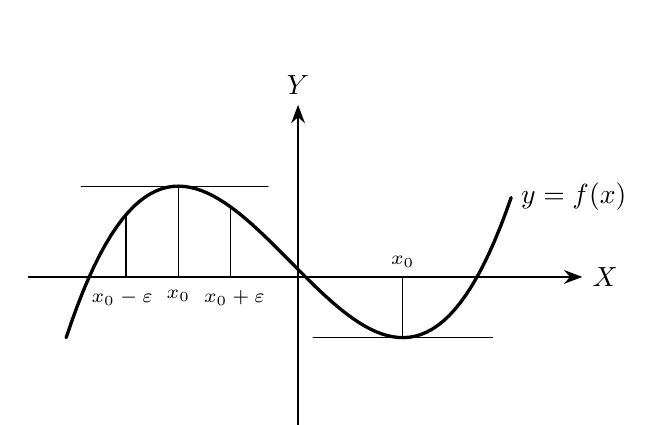
\begin{tikzpicture}[>=Stealth, scale=0.95, line cap=round, line join=round]
  \draw[->, thick] (-3.6, 0) -- (3.8, 0) node[right] {$X$};
  \draw[->, thick] (0, -2.1) -- (0, 2.3) node[above] {$Y$};

  % Explicit cubic with local max at x = -1.6 (y=1.214), local min at x = 1.4 (y=-0.811)
  % Left root at x ~ -2.79, clearing x_0-\varepsilon completely
  \draw[very thick, domain=-3.10:2.85, samples=80]
    plot (\x, {0.15*\x*\x*\x + 0.045*\x*\x - 1.008*\x + 0.10});
  \node[right] at (2.85, 1.07) {$y=f(x)$};

  % Horizontal tangents at extrema (matching original p.110)
  \draw[thin] (-2.9, 1.214) -- (-0.4, 1.214);
  \draw[thin] (0.2, -0.811) -- (2.6, -0.811);

  % Three vertical lines around local max x0 = -1.6 with generous spacing
  % f(-2.30) = 0.831, f(-1.60) = 1.214, f(-0.90) = 0.934
  \draw[thin] (-2.30, 0) -- (-2.30, 0.831);
  \draw[thin] (-1.60, 0) -- (-1.60, 1.214);
  \draw[thin] (-0.90, 0) -- (-0.90, 0.934);
  \node[below, font=\scriptsize] at (-2.35, -0.05) {$x_0-\varepsilon$};
  \node[below, font=\scriptsize] at (-1.60, -0.05) {$x_0$};
  \node[below, font=\scriptsize] at (-0.85, -0.05) {$x_0+\varepsilon$};

  % Vertical line at local min x0 = 1.4
  \draw[thin] (1.4, 0) node[above, font=\scriptsize] {$x_0$} -- (1.4, -0.811);
\end{tikzpicture}
\end{figure}

從上圖可看出所謂的極大、極小值，只是跟該函數在該點近傍的函數值做比較而已。它不一定是整個定義區間中的最大值或是最小值。我們可作出一個函數的圖形有二個以上的極大值：

\begin{figure}[H]
\centering
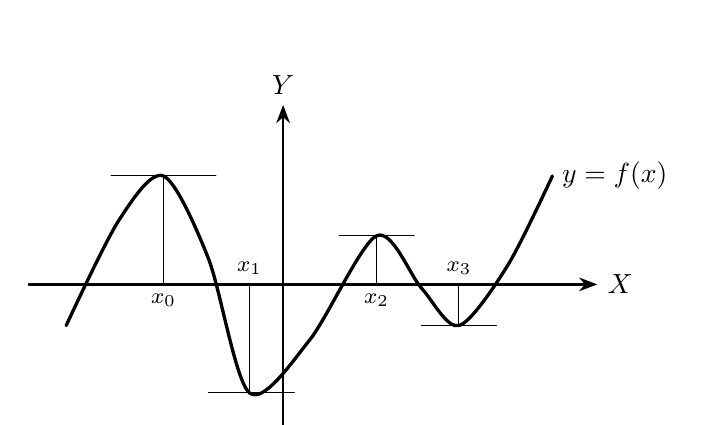
\begin{tikzpicture}[>=Stealth, scale=0.95, line cap=round, line join=round]
  \draw[->, thick] (-3.4, 0) -- (4.2, 0) node[right] {$X$};
  \draw[->, thick] (0, -2.0) -- (0, 2.4) node[above] {$Y$};

  % Smooth curve with 4 extrema: x0=-1.6 (max 1.4), x1=-0.45 (min -1.45), x2=1.25 (max 0.65), x3=2.35 (min -0.55)
  \draw[very thick, smooth] plot coordinates {
    (-2.9, -0.55) (-2.2, 0.85) (-1.6, 1.45) (-1.0, 0.35) (-0.45, -1.45)
    (0.35, -0.75) (1.25, 0.65) (1.85, -0.05) (2.35, -0.55) (3.0, 0.25) (3.6, 1.45)
  };
  \node[right] at (3.6, 1.45) {$y=f(x)$};

  % Horizontal tangent segments and vertical lines (matching original p.111)
  \draw[thin] (-2.3, 1.45) -- (-0.9, 1.45);
  \draw[thin] (-1.0, -1.45) -- (0.15, -1.45);
  \draw[thin] (0.75, 0.65) -- (1.75, 0.65);
  \draw[thin] (1.85, -0.55) -- (2.85, -0.55);

  \draw[thin] (-1.6, 0) node[below, font=\footnotesize] {$x_0$} -- (-1.6, 1.45);
  \draw[thin] (-0.45, 0) node[above, font=\footnotesize] {$x_1$} -- (-0.45, -1.45);
  \draw[thin] (1.25, 0) node[below, font=\footnotesize] {$x_2$} -- (1.25, 0.65);
  \draw[thin] (2.35, 0) node[above, font=\footnotesize] {$x_3$} -- (2.35, -0.55);
\end{tikzpicture}
\end{figure}

函數 $f(x)$ 在 $x_0, x_2$ 有極大值，但 $f(x_0) > f(x_2)$。

回頭再來看看函數 $f(x)$ 的泰勒展開式：
\begin{align*}
f(x+h) - f(x) &= f'(x)h + f''(x)\dfrac{h^2}{2!} + f'''(x)\dfrac{h^3}{3!} + \dots + f^{(n)}(x)\dfrac{h^n}{n!} \\
&= f'(x)h + h^2 \left( f''(x)\dfrac{1}{2!} + f'''(x)\dfrac{h}{3!} + \dots + f^{(n)}(x)\dfrac{h^{n-2}}{n!} \right)
\end{align*}
如果 $f(x)$ 的第一階導函數 $f'(x)$ 在某點 $x_0$ 取得 0 值，即 $f'(x_0)=0$ 則得
\begin{equation}
f(x_0+h) - f(x_0) = h^2 \left[ f''(x_0)\dfrac{1}{2!} + f'''(x_0)\dfrac{h}{3!} + \dots + f^{(n)}(x_0)\dfrac{h^{n-2}}{n!} \right] \label{eq:b6-2-4-extrema-1}
\end{equation}
當 $h$ 在很小很小的範圍內變動時，右邊有含 $h$ 的項數（不管 $f^{(i)}(x_0)$ 為正或負）皆為很小，因此 \eqref{eq:b6-2-4-extrema-1} 式中右邊為正或負，完全取定於 $f''(x_0)$ 為正或為負。如 $f''(x_0)$ 為正，則對任意小數 $h, f(x_0+h)-f(x_0) \ge 0$ 即 $f(x)$ 在 $x_0$ 有極小值；如果 $f''(x_0)$ 為負，則對任意小數 $h, f(x_0+h)-f(x_0) \le 0$ 即 $f(x)$ 在 $x_0$ 有極大值。因此，我們可得下面的定理：

\begin{theorem}[極值判別法]\label{thm:b6-2-extrema}
如果多項式函數 $f(x)$，對於一點 $x_0$，有
\[ \begin{cases} f'(x_0) = 0 \\ f''(x_0) < 0 \end{cases} \implies f(x) \text{ 在 } x_0 \text{ 有極大值} \]
如果
\[ \begin{cases} f'(x_0) = 0 \\ f''(x_0) > 0 \end{cases} \implies f(x) \text{ 在 } x_0 \text{ 有極小值} \]
\end{theorem}

\begin{example}\label{ex:b6-2-22}
令 $f(x)$ 為二次函數求極大、極小值。
\end{example}

\paragraph{【解】}
$f(x) = a_2 x^2 + a_1 x + a_0$
$f'(x) = 2a_2 x + a_1$
$f''(x) = 2a_2$
令 $f'(x) = 2a_2 x + a_1 = 0 \implies x = \dfrac{-a_1}{2a_2}$。
$f(x)$ 在 $x_0 = \dfrac{-a_1}{2a_2}$ 取極大或極小值。
如果 $a_2 > 0$，$f(x)$ 在 $x_0$ 有極小值，極小值為 $f\left(\dfrac{-a_1}{2a_2}\right)$。
如果 $a_2 < 0$，$f(x)$ 在 $x_0$ 有極大值，極大值為 $f\left(\dfrac{-a_1}{2a_2}\right)$。\hfill$\#$

\begin{example}\label{ex:b6-2-23}
$f(x)=x^2+2x+2$，求 $f(x)$ 的極大，極小值。
\end{example}

\paragraph{【解】}
$f'(x)=2x+2$。故 $2x+2=0 \implies x=-1$。
$f(x)$ 在 $x=-1$ 得極小值，極小值為 $f(-1)=1+2(-1)+2=1$。
各位很容易用配方法知
\[ f(x) = (x+1)^2+1 \ge 1 \qquad \text{當 } x=-1 \text{ 時 } f(x) \text{ 最小}=1 \]\hfill$\#$

\subsubsection*{作業 14}\label{hw:b6-2-14}
求 $f(x)=x^3+3x^2-x-3$ 之極大、極小值。

\subsubsection*{習題 II-4}\label{sec:b6-ex2-4}

\begin{enumerate}[label=\arabic*., leftmargin=2em]
  \item 試求下列各多項式的導函數：
  \begin{multicols}{2}
  \begin{enumerate}[label=(\roman*)]
    \item $x^4-3x^2+5$
    \item $x^5-3x^4+5x^2+7$
    \item $(x-1)^3(x+2)^2$
    \item $(x^2+1)^2(x-5)^3$
  \end{enumerate}
  \end{multicols}

  \item 試求下列各多項式的導數：
  \begin{enumerate}[label=(\roman*)]
    \item $f(x)=x^3-4x^2+5$ 求 $f'(1), f''(0), f'''(3), f^{(4)}(0)$。
    \item $f(x)=x^3(x^3-3x^2+6x+4)$，求 $f'(0), f''(0), f'''(0)$。
  \end{enumerate}

  \item 試把 $x^3+4x^2+5x-7$ 展開為 $x-2$ 的泰勒展開式。

  \item 給定 $f(x)=4x^3-3x^2-7x+5$
  \begin{enumerate}[label=(\roman*)]
    \item 試求 $f(x)$ 在 $x=-3$ 的泰勒展開式。
    \item 求 $f(-3.01)$ 至小數第 3 位。
  \end{enumerate}

  \item 已知 $f(x)=x^4+x^3+ax^2+bx-2=0$ 有 $x=1$ 的二重根，求 $a, b$。

  \item 已知 $f(x)=x^5-5x^3+5x+2=0$ 有重根，試解之。

  \item 已知下列各方程式有重根，試解之：
  \begin{enumerate}[label=(\roman*)]
    \item $x^4-6x^3+13x^2-12x+4=0$
    \item $x^4-x^3-3x^2+5x-2=0$
    \item $x^4+4x^3+10x^2+12x+9=0$
  \end{enumerate}

  \item 試問下列各方程式有重根時 $a$ 值如何？
  \begin{enumerate}[label=(\roman*)]
    \item $f(x)=x^3-3x+a=0$
    \item $f(x)=3x^4+4x^3-6x^2-12x+a=0$
  \end{enumerate}

  \item 試求下列各函數的極大、極小值：
  \begin{enumerate}[label=(\roman*)]
    \item $x^3-3x^2+4$
    \item $x^2(x+4)^2$
    \item $2x^3+x^2-8x+2$
  \end{enumerate}
\end{enumerate}

\subsection{*三次方程式、四次方程式的解法}\label{sec:b6-2-5}
\resetsectcounters

任意實係數一次方程式 $ax+b=0$ 之解為 $x=-\dfrac{b}{a}$，任意實係數二次方程式 $ax^2+bx+c=0$ 之解為 $x=\dfrac{-b \pm \sqrt{b^2-4ac}}{2a}$，那麼是否有一公式可以將任意三次方程式 $a_3 x^3 + a_2 x^2 + a_1 x + a_0 = 0$ 解出來呢？

在 16 世紀，對於三次方程式已有解法，通稱\textbf{卡丹解法}，四次方程式亦有公式解，至於五次方程式以上，已證出：

\begin{theorem}\label{thm:b6-2-abel-ruffini}
若 $n$ 為大於 4 之正整數，則必有不能開方解出之 $n$ 次方程式存在。
\end{theorem}

探究未知是人類求生存必然的活動，歸納已知的事實推廣到一般現象是我們習於操作的，但什麼樣的事實可以歸納？例如對一元的一次、二次、三次、四次方程式，若都可求得公式解，是否對五次以上亦做得到？利用代數方法已證明這是不可能的了。因為證明中用到較深一點的數學工具，證明的方法未能普遍授於眾人，這件不可能的事實到今天還不為眾所周知。這樣的事正像到今天還有不知多少人耗費他們的精力求做柏拉圖提出的名題，以直尺（無刻度的）及圓規三等分一個角一樣。並不是角不能三等分，這問題與所用的工具有關，工匠早就知道利用等分線段的方法準確地三等分一個角，而 Euclid 也早就揚棄柏拉圖的限制做出三等分來，但若要受柏拉圖所加的限制便是絕對做不到。它之不可能可以由方程式論的觀點來看，你若難以相信這件事，就請你在嘗試去做之前，花點精力認識一下這件事的證明過程，而如果你實在有需要三等分一個角，何不掙開柏拉圖給的限制，採用便利的工具？我們不必再為這個問題鑽牛角尖，而用我們的精力去尋求可能存在的另一些真理。

\subsubsection*{甲、一元三次方程式的解法}\label{subsec:b6-2-5-a}

設實係數三次方程式為
\begin{equation}
a_3 x^3 + a_2 x^2 + a_1 x + a_0 = 0 \label{eq:b6-2-5-1}
\end{equation}
以 $a_3$ 遍除各項得
\begin{equation}
x^3 + \dfrac{a_2}{a_3}x^2 + \dfrac{a_1}{a_3}x + \dfrac{a_0}{a_3} = 0 \label{eq:b6-2-5-2}
\end{equation}
(1) 與 (2) 有相同的根，故我們只考慮這樣的三次式
\begin{equation}
x^3 + bx^2 + cx + d = 0 \label{eq:b6-2-5-3}
\end{equation}
以 $x = z - \dfrac{b}{3}$ 代入，可得一新方程式
\begin{equation}
z^3 + pz + q = 0 \label{eq:b6-2-5-4}
\end{equation}
其中消去二次項，(4) 式中諸根減 $\dfrac{b}{3}$ 得 (3) 式中諸根，因此吾人只需解 (4) 式，令
\begin{equation}
z = u - \dfrac{p}{3u} \label{eq:b6-2-5-5}
\end{equation}
代入 (4)
\[ \left( u - \dfrac{p}{3u} \right)^3 + p\left( u - \dfrac{p}{3u} \right) + q = 0 \]
整理之，得
\begin{equation}
u^3 - \dfrac{p^3}{27u^3} + q = 0 \label{eq:b6-2-5-6}
\end{equation}
即
\begin{equation}
(u^3)^2 + qu^3 - \dfrac{p^3}{27} = 0 \label{eq:b6-2-5-7}
\end{equation}
視此為 $u^3$ 的二次式，利用公式得
\begin{align}
u^3 &= \dfrac{-q + \sqrt{q^2 + 4\frac{p^3}{27}}}{2} = -\dfrac{q}{2} + \sqrt{\dfrac{q^2}{4} + \dfrac{p^3}{27}} \label{eq:b6-2-5-8} \\
u^3 &= -\dfrac{q}{2} - \sqrt{\dfrac{q^2}{4} + \dfrac{p^3}{27}} \label{eq:b6-2-5-9}
\end{align}
令
\begin{align*}
\alpha &= \sqrt[3]{-\dfrac{q}{2} + \sqrt{\dfrac{q^2}{4} + \dfrac{p^3}{27}}} \tag{I} \\
\beta &= \sqrt[3]{-\dfrac{q}{2} - \sqrt{\dfrac{q^2}{4} + \dfrac{p^3}{27}}} \tag{II}
\end{align*}
設 $\omega$ 為 $x^3=1$ 之複數根，$1+\omega+\omega^2=0$。\\
得 \eqref{eq:b6-2-5-8} 中 $u$ 有三解：$\alpha, \alpha\omega, \alpha\omega^2$。\\
\eqref{eq:b6-2-5-9} 中 $u$ 有三解：$\beta, \beta\omega, \beta\omega^2$。\\
代入 \eqref{eq:b6-2-5-5} 得
\[ z = \alpha+\beta, \quad \omega\alpha+\omega^2\beta, \quad \omega^2\alpha+\omega\beta \]
此即為三次式的三根。

\begin{example}\label{ex:b6-2-24}
試解 $x^3-6x^2+6x-2=0$。
\end{example}

\paragraph{【解】}
令 $y=x-2$ 代入得 $y^3-6y-6=0$ 其中 $p=-6, q=-6$。
代入公式 (I), (II) 得
\[ \alpha = \sqrt[3]{4}, \quad \beta = \sqrt[3]{2} \]
所以
\[ y = \sqrt[3]{4}+\sqrt[3]{2}, \quad \sqrt[3]{4}\omega+\sqrt[3]{2}\omega^2, \quad \sqrt[3]{4}\omega^2+\sqrt[3]{2}\omega \]
故原方程式之根為 $2+\sqrt[3]{4}+\sqrt[3]{2}, 2+\sqrt[3]{4}\omega+\sqrt[3]{2}\omega^2, 2+\sqrt[3]{4}\omega^2+\sqrt[3]{2}\omega$。\hfill$\#$

\subsubsection*{乙、一元四次方程式的解法}\label{subsec:b6-2-5-b}

設實係數一元四次方程式為
\begin{equation}
x^4 + ax^3 + bx^2 + cx + d = 0 \label{eq:b6-2-5-10}
\end{equation}
於 \eqref{eq:b6-2-5-10} 左右兩端各加 $(px+q)^2$，得
\begin{equation}
x^4 + ax^3 + bx^2 + cx + d + (px+q)^2 = (px+q)^2 \label{eq:b6-2-5-11}
\end{equation}
假設 \eqref{eq:b6-2-5-11} 左邊為完全平方 $= \left(x^2 + \dfrac{a}{2}x + k\right)^2$。展開比較係數得
\begin{equation}
2k + \dfrac{a^2}{4} = b + p^2, \quad ak = c + 2pq, \quad k^2 = d + q^2 \label{eq:b6-2-5-12}
\end{equation}
故
\[ p^2 = 2k + \dfrac{a^2}{4} - b, \quad q^2 = k^2 - d, \quad 2pq = ak - c \]
得
\[ 4(k^2-d)\left(2k+\dfrac{a^2}{4}-b\right) = (ak-c)^2 \]
此為 $k$ 的三次方程式：
\[ 8k^3 - 4bk^2 - 2(ac-4d)k + 4bd - a^2d - c^2 = 0 \]
求得實數解 $k$ 後，利用 \eqref{eq:b6-2-5-12} 決定 $p, q$ 值。又由 \eqref{eq:b6-2-5-10}, \eqref{eq:b6-2-5-11} 知
\[ \left(x^2 + \dfrac{a}{2}x + k\right)^2 = (px+q)^2 \]
故原方程式可分解為二個二次方程式，為
\begin{align*}
x^2 + \dfrac{a}{2}x + k - px - q &= 0 \\
x^2 + \dfrac{a}{2}x + k + px + q &= 0
\end{align*}
此二方程之解，即為原方程式之解。

\begin{example}\label{ex:b6-2-25}
試解四次方程式
\[ x^4 + 8x^3 + 12x^2 - 11x + 2 = 0 \]
\end{example}

\paragraph{【解】}
\setcounter{equation}{0}%
於原方程式兩端各加以 $(px+q)^2$ 得
\begin{equation}
x^4 + 8x^3 + 12x^2 - 11x + 2 + (px+q)^2 = (px+q)^2 \label{eq:b6-2-5-ex2-1}
\end{equation}
假設
\begin{equation}
x^4 + 8x^3 + 12x^2 - 11x + 2 + p^2x^2 + 2pqx + q^2 = (x^2+4x+k)^2 \label{eq:b6-2-5-ex2-2}
\end{equation}
比較 \eqref{eq:b6-2-5-ex2-2} 式左右兩端係數，得
\begin{equation}
16 + 2k = 12 + p^2, \quad 8k = 2pq - 11, \quad k^2 = 2 + q^2 \label{eq:b6-2-5-ex2-3}
\end{equation}
消去 $p, q$ 得 $k$ 之三次方程式：
\begin{equation}
8k^3 - 48k^2 - 192k - 153 = 0 \label{eq:b6-2-5-ex2-4}
\end{equation}
利用公式解 (4)，得 $k$ 之實根為 $k = -\dfrac{3}{2}$。代入 \eqref{eq:b6-2-5-ex2-3} 得
\[ p = 1, \quad q = -\dfrac{1}{2} \]
以 $k, p, q$ 之值代入 \eqref{eq:b6-2-5-ex2-1}, \eqref{eq:b6-2-5-ex2-2} 得
\[ \left(x^2+4x-\dfrac{3}{2}\right)^2 = \left(x-\dfrac{1}{2}\right)^2 \]
故得
\[ \begin{cases}
x^2 + 3x - 1 = 0 \\
x^2 + 5x - 2 = 0
\end{cases} \]
解之得原方程式四根為
\[ \dfrac{-3 \pm \sqrt{13}}{2} \quad \text{及} \quad \dfrac{-5 \pm \sqrt{33}}{2} \]\hfill$\#$

\subsubsection*{習題 II-5}\label{sec:b6-ex2-5}

\begin{enumerate}[label=\arabic*., leftmargin=2em]
  \item 試解 $x^3-6x+4=0$。
  \item 試解 $x^3-3x^2-3x-1=0$。
  \item 試解 $x^3-2x^2+1=0$。
  \item 試解 $x^3-12x+65=0$。
  \item 試解 $x^3-9x+28=0$。
  \item 設 $x^3+px+r=0$ 的三根皆為實根，試證 $p, r$ 為負，且 $-4p^3r > 27r$\phantomsection\label{note:b6-ch2-p117-cubic-ineq}\footnote{【原書註記】：依判別式條件，原書所列不等式 $-4p^3 > 27r^2$ 印損為 $-4p^3r > 27r$。}。
  \item 試解下列四次方程式：
  \begin{multicols}{2}
  \begin{enumerate}[label=(\roman*)]
    \item $x^4+2x^3+14x+15=0$
    \item $x^4-12x-5=0$
    \item $x^4-12x^2+24x+140=0$
    \item $x^4-14x^3+71x^2-154x+120=0$
    \item $x^4-2x^3-5x^2+10x-3=0$
    \item $x^4+8x^3+22x^2+32x+21=0$
  \end{enumerate}
  \end{multicols}
\end{enumerate}

\phantomsection
\subsection*{附錄 III\quad 結式判別式與史篤姆定理}\label{sec:b6-app3}
\addcontentsline{toc}{subsection}{\texorpdfstring{附錄 III\quad 結式判別式與史篤姆定理}{附錄 III 結式判別式與史篤姆定理}}
\resetsectcounters

\subsubsection*{1. 結式}\label{subsec:b6-app3-1}

設二個一元方程式為
\begin{align}
f(x) &= a_0 x^3 + a_1 x^2 + a_2 x + a_3 = 0 \label{eq:b6-app3-1} \\
g(x) &= b_0 x^2 + b_1 x + b_2 = 0 \label{eq:b6-app3-2}
\end{align}
\eqref{eq:b6-app3-1} 式分別乘以 $x, 1$，\eqref{eq:b6-app3-2} 式分別乘以 $x^2, x, 1$ 得
\begin{equation}
\left\{\begin{aligned}
a_0 x^4 + a_1 x^3 + a_2 x^2 + a_3 x &= 0 \\
a_1 x^3 + a_1 x^2 + a_2 x + a_3 &= 0 \\
b_0 x^4 + b_1 x^3 + b_2 x^2 &= 0 \\
b_0 x^3 + b_1 x^2 + b_2 x &= 0 \\
b_0 x^2 + b_1 x + b_2 &= 0
\end{aligned}\right. \label{eq:b6-app3-6}
\end{equation}
把 (3) 式看做 $x^4, x^3, x^2, x, 1$ 的五元一次聯立方程式，如果 (3) 有共同解，由克萊瑪法則知其係數行列式
\[ D = \begin{vmatrix}
a_0 & a_1 & a_2 & a_3 & 0 \\
0 & a_0 & a_1 & a_2 & a_3 \\
b_0 & b_1 & b_2 & 0 & 0 \\
0 & b_0 & b_1 & b_2 & 0 \\
0 & 0 & b_0 & b_1 & b_2
\end{vmatrix} = 0 \]
反之如果 $D=0$，由行列式的運算，得
\[ 0 = \begin{vmatrix}
a_0 & a_1 & a_2 & a_3 & x(a_0 x^3 + a_1 x^2 + a_2 x + a_3) \\
0 & a_0 & a_1 & a_2 & a_0 x^3 + a_1 x^2 + a_2 x + a_3 \\
b_0 & b_1 & b_2 & 0 & x^2(b_0 x^2 + b_1 x + b_2) \\
0 & b_0 & b_1 & b_2 & x(b_0 x^2 + b_1 x + b_2) \\
0 & 0 & b_0 & b_1 & b_0 x^2 + b_1 x + b_2
\end{vmatrix} \]
設 $\alpha_1, \alpha_2, \alpha_3, \alpha_4, \alpha_5$ 分別為 $D$ 中第五列的餘因式，則得
\begin{equation}
0 \equiv D \equiv (\alpha_1 x + \alpha_2) f(x) + (\alpha_3 x^2 + \alpha_4 x + \alpha_5) g(x) \label{eq:b6-app3-4}
\end{equation}
由 (4) 式知，如果 $(x-B)$ 為 $f(x)$ 的一個因式，則 $x-B$ 必為 $(\alpha_3 x^2 + \alpha_4 x + \alpha_5) g(x)$ 的因式。因 $f(x)=0$ 有三個根，而 $\alpha_3 x^2 + \alpha_4 x + \alpha_5 = 0$ 為二次方程式，故 $f(x)=0$ 與 $g(x)=0$ 必共根。

\begin{definition}\label{def:b6-app3-resultant}
設 $f(x) = a_0 x^n + a_1 x^{n-1} + \dots + a_n = 0, g(x) = b_0 x^m + b_1 x^{m-1} + \dots + b_m = 0$ 分別為 $n, m$ 次方程式，則它們的\textbf{結式} $D(f, g)$ 為 $m+n$ 階行列式：
\[ D(f, g) = \begin{vmatrix}
a_0 & a_1 & a_2 & \dots & a_n & 0 & 0 & \dots & 0 \\
0 & a_0 & a_1 & \dots & a_{n-1} & a_n & 0 & \dots & 0 \\
0 & 0 & \dots & \dots & \dots & \dots & \dots & \dots & \dots \\
0 & 0 & \dots & 0 & a_0 & a_1 & a_2 & \dots & a_n \\
b_0 & b_1 & \dots & \dots & \dots & b_m & 0 & \dots & 0 \\
0 & b_0 & b_1 & \dots & \dots & \dots & b_{m-1} & b_m & 0 \\
\dots & \dots & \dots & \dots & \dots & \dots & \dots & \dots & \dots \\
0 & \dots & 0 & b_0 & b_1 & \dots & \dots & \dots & b_m
\end{vmatrix} \]
\end{definition}

從上述的討論可得：

\begin{theorem}\label{thm:b6-app3-resultant-roots}
設 $f(x) = a_0 x^n + \dots + a_n = 0, g(x) = b_0 x^m + \dots + b_m = 0$ 分別為 $n, m$ 次方程式。則 $f(x)=0, g(x)=0$ 有共根之充要條件為 $D(f, g) = 0$。
\end{theorem}

\begin{example}\label{ex:b6-app3-1}
試證 $x^2+3x+2=0$ 與 $x+1=0$ 有共根。
\end{example}

\paragraph{【解】}
$D = \begin{vmatrix} 1 & 3 & 2 \\ 1 & 1 & 0 \\ 0 & 1 & 1 \end{vmatrix} = 1 + 2 - 3 = 0$。故 $x^2+3x+2=0$ 與 $x+1=0$ 有共根。\\
事實上我們很容易看出 $x^2+3x+2 = (x+1)(x+2)$ 有一根為 $-1$。\hfill$\#$

\subsubsection*{2. 判別式}\label{subsec:b6-app3-2}

\begin{definition}\label{def:b6-app3-discriminant}
給一方程式 $f(x) = a_0 x^n + a_1 x^{n-1} + \dots + a_n = 0$ ($a_0 \ne 0$)，$D(f, f')/a_0$ 稱為 $f(x)$ 的\textbf{判別式}。
\end{definition}

我們從上節中知 $f(x)=0$ 與 $f'(x)=0$ 有共根之充要條件是 $D(f, f') = 0$，因此我們能從 $D(f) = D(f, f')/a_0$ 中知 $f(x)=0$ 有沒有重根。

\begin{example}\label{ex:b6-app3-2}
設二次方程式為 $f(x)=a_0 x^2 + a_1 x + a_2 = 0$，則 $f'(x)=2a_0 x + a_1$。
\end{example}

得
\begin{align*}
D &= \dfrac{1}{a_0} D(f, f') = \dfrac{1}{a_0} \begin{vmatrix}
a_0 & a_1 & a_2 \\
2a_0 & a_1 & 0 \\
0 & 2a_0 & a_1
\end{vmatrix} \\
&= \dfrac{1}{a_0}(a_0 a_1^2 + 4a_0^2 a_2 - 2a_0 a_1^2) = -(a_1^2 - 4a_0 a_2)
\end{align*}
故 $f(x)=0$ 有重根之充要條件為 $a_1^2 - 4a_0 a_2 = 0$。\hfill$\#$

一般的判別式有下列定理：

\begin{theorem}\label{thm:b6-app3-disc-roots}
設 $\beta_1, \beta_2, \dots, \beta_n$ 為 $f(x) = a_0 x^n + \dots + a_n = 0$ 的 $n$ 個根，則 $f(x)=0$ 的判別式為
\[ D(f) = C(\beta_1-\beta_2)^2 \dots (\beta_1-\beta_n)^2 \dots (\beta_i-\beta_j)^2 \dots (\beta_{n-1}-\beta_n)^2 \]
即 $D(f) = C \prod_{i<j} (\beta_i-\beta_j)^2$，$C$ 為常數。
\end{theorem}

\subsubsection*{3. 史篤姆 (Sturm's) 定理}\label{subsec:b6-app3-3}

設一方程式 $f(x)=0$ 無重根，$f_1(x)=f'(x)$ 為 $f(x)$ 的第一階導函數。令
\begin{equation}
f(x) \equiv q_1 f_1(x) - f_2(x) \label{eq:b6-app3-sturm-1}
\end{equation}
$q_1(x)$ 為 $f(x)$ 被 $f_1(x)$ 除的商，而 $-f_2(x)$ 為其餘式，同理令
\begin{align}
f_1(x) &\equiv q_2 f_2(x) - f_3(x) \label{eq:b6-app3-sturm-2} \\
f_{m-2}(x) &\equiv q_{m-1} f_{m-1}(x) - f_m(x) \label{eq:b6-app3-sturm-3}
\end{align}
而設 $-f_m(x)$ 為常數。因為 $f(x)$ 無重根故這樣輾轉相除的最後項 $f_m(x)$ 不等於 0。這樣的一組函數
\[ f(x), f_1(x), f_2(x), \dots, f_m(x) \]
稱為 $f(x)$ 的 \textbf{Sturm's 函數}。

設取任二數 $a, b$ ($a < b$) 考慮下列數列：
\begin{align}
f(a), f_1(a), f_2(a), \dots, f_m(a) \label{eq:b6-app3-sturm-a} \\
f(b), f_1(b), f_2(b), \dots, f_m(b) \label{eq:b6-app3-sturm-b}
\end{align}
設 \eqref{eq:b6-app3-sturm-a} 中相鄰二數變號的個數為 $n$，\eqref{eq:b6-app3-sturm-b} 中相鄰二數變號的個數為 $m$，則

\begin{theorem}[Sturm 定理]\label{thm:b6-app3-sturm}
設 $f(x)=0$，有 $l$ 個根落在 $[a, b]$ 中，則
\[ l = n - m \]
（定理的證明從略）
\end{theorem}

\begin{example}\label{ex:b6-app3-3}
$f(x) = x^3 + 3x^2 - 4x + 1 = 0$
\end{example}

\paragraph{【解】}
$f'(x) = f_1(x) = 3x^2 + 6x - 4$。用輾轉相除法得 $f(x)$ 的 Sturm 函數為
\begin{align*}
f(x) &= x^3 + 3x^2 - 4x + 1 \\
f_1(x) &= 3x^2 + 6x - 4 \\
f_2(x) &= 2x - 1 \\
f_3(x) &= 1
\end{align*}
(1)
\begin{center}
\renewcommand{\arraystretch}{1.3}
\begin{tabular}{c|c|c|c|c|l}
& $f(x)$ & $f_1(x)$ & $f_2(x)$ & $f_3(x)$ & \\
\hline
$x = -\infty$ & $-$ & $+$ & $-$ & $+$ & 三個變號 \\
$x = 0$       & $+$ & $-$ & $-$ & $+$ & 二個變號 \\
$x = \infty$  & $+$ & $+$ & $+$ & $+$ & 無變號
\end{tabular}
\end{center}
故知 $(-\infty, 0]$ 中有一根，$[0, \infty)$ 有二根。

(2)
\begin{center}
\renewcommand{\arraystretch}{1.3}
\begin{tabular}{c|c|c|c|c|l}
& $f(x)$ & $f_1(x)$ & $f_2(x)$ & $f_3(x)$ & \\
\hline
$x = 0$ & $+$ & $-$ & $-$ & $+$ & 二個變號 \\
$x = 1$ & $+$ & $+$ & $+$ & $+$ & 無變號
\end{tabular}
\end{center}
故知 $f(x)$ 的二正根落在 $[0, 1]$ 間。\hfill$\#$


\end{document}
